\chapter{Taylor series integration} %Last updated 18-05-2016
\label{ch:tsi}
\acf{TSI} is different from the previously mentioned integrators, because it only uses the information at the current point to predict the next point. However, it does this using higher order derivatives at that point. These higher order derivatives have to be obtained as a function of the current state and the first order state derivatives. As soon as the $K^{th}$ order derivative as been found, a Taylor Series can be set up to determine the next state as a function of the chosen step-size. This is all explained and described in more detail in \Cref{sec:genTsiTheory}. In this thesis, \ac{TSI} is the main focus of the analysis. The performance with respect to the \ac{RKF} integrators is tested. In order to be able to do this for the given model, a number of equation sets can be identified which have to be written in such a format that it can be used by \ac{TSI}. These are described, and where needed derived, in \Cref{sec:assEq}.

\section{General theory}
\label{sec:genTsiTheory}
\ac{TSI} has been used to solve ordinary differential equations since the early 1960s \citep{scott2008high}. However, the first modern implementation of \ac{TSI} in a space trajectory problem was provided by \cite{montenbruck1992numerical}. \cite{scott2008high} were able to implement this \ac{TSI} method into the SNAP trajectory propagator which is the implementation that is used in this thesis. The method is described in \Cref{subsec:workTsi} and the used step-size method is discussed in \Cref{subsec:stepSizeTsi}. This step-size sometimes has to be reduced if a new section in the temperature or the drag coefficient model is reached. A root finding method is described in \Cref{subsec:handlingModelSections} that can be used to determine at what step-size the next section is reached.



\subsection{Workings of \ac{TSI}}
\label{subsec:workTsi}
The formulation used in this thesis is based on the one used by \cite{scott2008high}. 

%In \cite{scott2008high} an example situation is used to describe the \ac{TSI} method: the thrust-less motion around a central body. For consistency the same example and formulation will be used. 


\ac{TSI} uses the current state and its derivatives to determine the next state by computing its Taylor Series described in \Cref{eq:general_taylor}. The state vector is represented by $\mathbf{X}$ with the corresponding vector for the initial conditions $\mathbf{X}_{0}$. Each of the variables can at any point be represented by $x_{n}\left(t\right)$. For a given step-size $h$ and an order $K \in \mathbb{R}$ (chosen by the user) the updated state $x_{n}\left(t+h\right)$ can be represented by the Taylor Series with $n=1,\dots,7$ in this case (7 variables: three position, three velocity and one mass). The exact solution is obtained by adding $T_{n,K}$, which is the truncation error for the $n^{th}$ variable using K terms. 

\nomenclature[Rb4]{$\mathbf{X}$}{State vector \nomunit{-}}
\nomenclature[Rb1]{$x_{n}$}{n$^{th}$ state variable \nomunit{-}}
\nomenclature[Ra9]{$T_{n,k}$}{Truncation error \nomunit{-}}
\nomenclature[Ra4]{$K$}{Maximum order \nomunit{-}}
\nomenclature[Ra3]{$k$}{Order derivative \nomunit{-}}


\begin{equation} \label{eq:general_taylor}
x_{n}\left(t+h\right)=\displaystyle\sum_{k=0}^{K}\dfrac{x_{n}^{\left(k\right)}\left(t\right)}{k!}h^{k} \quad + \quad	T_{n,K}
\end{equation}

This particular \ac{TSI} method uses recurrence relations to determine the $k^{th}$ order derivatives and only requires the current state ($x_{n}$) and its first derivatives ($x'_{n} = u_{n}$). Each recurrence relation describes a certain operation in the state derivative, such as: multiplication, division, power, exponential, sines and cosines. \Cref{eq:rec_rel} shows the recurrence relations for multiplication ($w\left(t\right)=f\left(t\right)g\left(t\right)$) and division ($w\left(t\right)=\dfrac{f\left(t\right)}{g\left(t\right)}$) respectively (the other operations are described later in this chapter when they are required).

\nomenclature[Rb1]{$x_{n}$}{Auxiliary equation \nomunit{-}}
\nomenclature[Rb0]{$u_{n}$}{Auxiliary derivative \nomunit{-}}
\nomenclature[Rb1]{$w_{n,i}$}{Auxiliary function \nomunit{-}}
\nomenclature[Ra1]{$f_{n}$}{Auxiliary placeholder function \nomunit{-}}
\nomenclature[Ra1]{$g_{n}$}{Auxiliary placeholder function \nomunit{-}}

\begin{equation} \label{eq:rec_rel}
\begin{split}
&\text{For multiplications} \quad W\left(k\right)=\displaystyle\sum_{j=0}^{k}F\left(j\right)G\left(k-j\right)\\
&\text{For divisions} \quad W\left(k\right)=\dfrac{1}{g\left(t_{0}\right)}\left[F\left(k\right)-\displaystyle\sum_{j=1}^{k} G\left(j\right)W\left(k-j\right)\right]\\
& Both \ with \quad W\left(k\right)=\dfrac{w^{\left(k\right)}\left(t_{0}\right)}{k!}, \quad F\left(j\right)=\dfrac{f^{\left(j\right)}\left(t_{0}\right)}{j!} \quad \text{and} \quad G\left(k-j\right)=\dfrac{g^{\left(k-j\right)}\left(t_{0}\right)}{\left(k-j\right)!}\\
\end{split}
\end{equation}

Here, both $f\left(t\right)$ and $g\left(t\right)$ are place-holder functions and $w\left(t\right)$ is called the auxiliary function which replaces the respective operation. Sometimes, the state derivative functions can be rather complex and have many operations intertwined. One can then choose to introduce extra variables to simplify the derivatives and reduce the number of operations in that particular derivative. These extra variables together with the expression that they replace then form the auxiliary equations. A random example is shown in \Cref{eq:auxEqExample}.

\begin{equation} \label{eq:auxEqExample}
\begin{split}
x'_{4} &= u_{4} = 2x_{1}+\dfrac{\left(x_{3}x_{1}+x_{2}x_{3}\right)}{x_{4}} \\
x_{8} &= x_{3}x_{1}+x_{2}x_{3} \\
\end{split}
\end{equation}

However, now that the extra variable $x_{8}$ is introduced, the derivative of the corresponding auxiliary equations has to be described as well (see \Cref{eq:auxDerExample}, which in turn will use auxiliary functions to determine the $k^{th}$ derivative of $x_{8}$.

\begin{equation} \label{eq:auxDerExample}
\begin{split}
x'_{4} &= u_{4} = 2x_{1}+\dfrac{x_{8}}{x_{4}} \\
x'_{8} &= u_{8} =  x'_{3}x_{1}+x_{3}x'_{1}+x'_{2}x_{3}+x_{2}x'_{3} = u_{3}x_{1}+x_{3}u_{1}+u_{2}x_{3}+x_{2}u_{3} \\
\end{split}
\end{equation}

At this point it should be emphasised that using auxiliary equations and derivatives is a choice. It is not required to make \ac{TSI} work. Sometimes it can be easier to introduce auxiliary equations because it makes the problem more comprehensible but this could introduce errors because all auxiliary equations also require auxiliary derivatives, which might not be easy to find. In those cases it could be more useful to just leave the state derivatives as they are and write more auxiliary functions instead. This all depends on the problem and the preference of the user. 


Now let $u_{n}^{\left(k-1\right)}=x_{n}^{k}$ for $k=1,\dots,K$, then $\dfrac{u_{n}^{\left(k-1\right)}}{\left(k-1\right)!}=\dfrac{x_{n}^{k}}{\left(k-1\right)!}$, and also $\dfrac{x_{n}^{k}}{k!}=X_{n}\left(k\right)$. Combining this results in \Cref{eq:def_u}.

\begin{equation} \label{eq:def_u}
U_{n}\left(k-1\right)=kX_{n}\left(k\right)\Rightarrow X_{n}\left(k\right)=\dfrac{U_{n}\left(k-1\right)}{k}
\end{equation}

\nomenclature[Rb3]{$X$}{Taylor Series coefficient (also $X_{n}$) \nomunit{-}}

The $X_{n}\left(k\right)$ are also known as the Taylor Series coefficients of the $n^{th}$ variable for the $k^{th}$ order derivative. Also, $U_{n}\left(k\right)$ are the recurrence relation expressions for the $n^{th}$ variable which consist of all the reduced auxiliary functions ($W\left(k\right)$) that form that derivative. 


Using the expression described in \Cref{eq:def_u} all Taylor Series coefficients can be found. Then \Cref{eq:general_taylor} can be used to determine the next state values at time $t+h$ for the known previous parameter values at time $t$. The same can then be done to determine the values at the time-step after that using the state values at $t+h$, etc. Going through all these different time-steps results in the final integration. 

\subsection{Step-size}
\label{subsec:stepSizeTsi}
The step-size used for \ac{TSI} can be either set as a constant value by the user or determined using a step-size controller, giving it the variable step-size properties, which is done in this thesis. The chosen step-size method was based on the recommendation of both \cite{scott2008high} and \cite{bergsma2015application} and directly uses the chosen (or preferred) local error tolerance $\tau$ to determine the next step size. This method assures that the step-size is small enough such that all variables satisfy the error condition directly. The step-size is determined using a so-called fixed-point iteration performed using \Cref{eq:fix_point_it}. The initial step-size $h_{1}$ can be chosen to be the current step-size $h$ as an easy estimate. Then the iteration is performed over $l$ until a certain required convergence is reached.



\begin{equation} \label{eq:fix_point_it}
h_{l+1}=exp\left(\dfrac{1}{K-1}ln\left[\dfrac{\tau}{\begin{vmatrix}
X_{n}\left(K-1\right)
\end{vmatrix}+K\begin{vmatrix}
X_{n}\left(K\right)
\end{vmatrix}h_{l}}\right]\right)
\end{equation}

This is then done for all variables and the smallest required step-size is chosen, which is then used to determine the next step-size through $h_{next}=\eta h_{chosen}$, where $\eta$ is the chosen step multiplication factor which has to be smaller than 1. 

\nomenclature[Ga3]{$\eta$}{Step multiplication factor \nomunit{-}}
\nomenclature[Ga3]{$\tau$}{Local error tolerance \nomunit{-}}

\subsection{Handling model sections}
\label{subsec:handlingModelSections}
For both the temperature and drag coefficient models, different sections have been identified with different behaviours. Each of these sections was fitted with a polynomial approximation as described in \Cref{sec:dragModel}. Because \ac{TSI} only uses data available at the current point, it could be that if the step-size is allowed to be too large, the section boundary for one of these models is crossed. At that point, the step-size has to be adjusted such that it stops at the start of the next section. This way, the next time step will start at the next model section. This also means that these sections do not necessarily have to be connected, which means that \ac{TSI} would be able to handle discontinuities in the model as well, should those occur. \\
This section boundary is found using a root finding method. The method used in this research is based on the method described in \cite{bergsma2015application}. \\

\noindent
First, the simulation program has to determine if the newly computed parameter (either Mach number or altitude) has indeed moved into the new section. This can be done using the section limits as shown by \Cref{eq:limitFunction} which is called the limit function. From now on, the equations will be written for the altitude, but the same expressions hold for the Mach number.

\begin{equation} \label{eq:limitFunction}
f = h-h_{limit}
\end{equation}

\nomenclature[Ra1]{$f$}{Limit function \nomunit{-}}

\noindent
Because this research is based on an ascent trajectory, a new section is reached if the altitude is higher than the lower limit altitude of that section. Therefore, if $f$ > 0 a new section has been reached, and the root finding method should be used to get the value of $f$ back to zero and thus identify the step-size at which the root of $f$ is located.\\

\noindent
At the start of the root finding procedure, two points can be identified. The first point is the starting point of the \ac{MAV} at the beginning of the integration step and the second point is the proposed end point of the \ac{MAV} as suggested by the current step-size. If the new section has been reached it means that the point that the \ac{MAV} is coming from has a limit function value that is below zero, or $f_{From}$ < 0. The mission time at that point is given by $t_{From}$. This is the original mission time ($t_{original}$) at the start of the integration and it is therefore the goal to find $h_{req}$ (required step-size) such that $t_{original}+h_{req}$ results in the final limit function value, $f_{new}$ = 0. The mission time at the second point (where the \ac{MAV} was headed when the section was crossed) is given by $t_{To}$ with the corresponding $f_{To}$ > 0. This means that $f_{new}$ and $t_{new}$ are located somewhere between these original points. The method described by \cite{bergsma2015application} should result in a spiralling motion that slowly converges to the root. This means that the root finding method is always evaluated from the "from" point to the "to" point, irrespective of on which side of the root the next starting point is. \\

\noindent
The first step is to determine the altitude derivative at the current "from" point, or $\dot{f}_{From}$. If the Taylor Series coefficients for the altitude (in this case) are available, then the derivative can directly be computed by combining \Cref{eq:general_taylor,eq:def_u} resulting in \Cref{eq:fFromDot}. Otherwise, the derivative has to be comprised of other known derivatives.

\begin{equation}\label{eq:fFromDot}
\dot{f}_{From} \approx \displaystyle\sum_{k=1}^{K}kX\left(k\right) h^{k-1}
\end{equation}

\noindent
Next, the coefficient of the root finding curve, $\alpha$, has to be determined. This coefficient is effectively $\dfrac{\ddot{f}_{From}}{2}$ and is computed using \Cref{eq:alphaForRoot}.

\begin{equation} \label{eq:alphaForRoot}
\alpha = \dfrac{f_{To}-f_{From}}{\left(t_{To}-t_{From}\right)^{2}}-\dfrac{\dot{f}_{From}}{t_{To}-t_{From}}
\end{equation}

\nomenclature[Ga1]{$\alpha$}{Root finding curve coefficient \nomunit{-}}

\noindent
With this coefficient it is possible to compute the new time of the newly computed point. This point is called the new from point because no matter if this point is before of after the root of the limit function, that point will be used as the starting or "from" point for the next point computation. This is why this time is called $t_{From,new}$ and is computed using \Cref{eq:tFromNew}. This equation has a plus sign in front of the square root because the next section has been reached when $f$ > 0.

\begin{equation} \label{eq:tFromNew}
t_{From,new} = t_{From}+\dfrac{\left(-\dot{f}_{From}+\sqrt{\dot{f}_{From}^{2}+4\alpha f_{From}}\right)}{2\alpha}
\end{equation}

\noindent
Now that the new time is known, the step-size can be computed by simply taking the difference between the original time and the new time. With this new step-size, the Taylor Series coefficients can be used as per \Cref{eq:general_taylor} to determine the new altitude at that new "from" point. This means that, using \Cref{eq:limitFunction} the new limit function value $f_{From,new}$ = $h_{From,new}$-$h_{limit}$. If this $f_{From,new}$ value is zero it means that the section boundary has been found and the newly computed step-size is the step-size that should be used. However, if $f_{From,new}$ is on the other side of the root compared to $f_{From}$ then the "from" and "to" points have to be updated. The conditions are shown in \Cref{eq:updatedPointsRoot}.

\begin{equation}\label{eq:updatedPointsRoot}
\begin{split}
\text{If the signs of }f_{From}\text{ and }f_{From,new}\text{ are oposite}&\Rightarrow\begin{cases}
f_{To}=f_{From}\\
t_{To}=t_{From} \\
f_{From}=f_{From,new}\\
t_{From}=t_{From,new} \\ 
\end{cases}\\
\text{If the signs of }f_{From}\text{ and }f_{From,new}\text{ are the same}&\Rightarrow\begin{cases}
f_{To}=f_{To} \quad \text{  Remains the same}\\
t_{To}=t_{To} \quad \text{  Remains the same}\\
f_{From}=f_{From,new}\\
t_{From}=t_{From,new} \\ 
\end{cases}\\
\end{split}
\end{equation}

\noindent
With this, the root finding process can be started again at the first step (so starting at \Cref{eq:fFromDot}).\\

\noindent
However, the condition that $f_{From,new}$ should be equal to zero before the root finding method is satisfied and the new step-size can be accepted is not realistic. This is why two conditions have to be met instead. $f_{From,new}\geq 0$ and $f_{From,new}\leq 1\cdot10^{-6}$. This means that $f_{From,new}$ has to be within an accuracy of 1 cm for the altitude and within a Mach accuracy of 1$\cdot$10$^{-6}$. If both these cases are met, it is assured that the next section will be used in the next time step calculation, because the section limits have always been set at the beginning of the section.  


%This is where the root finding method used should be described!
%\textbf{\textcolor{red}{This section still has to be added!!}}


\section{Associated equations}
\label{sec:assEq}
In order for \ac{TSI} to be implemented, the state derivatives have to be modelled as a set of continuous functions which are a function of the state only. This can be done in different ways. In this case, three cases were tested: two Cartesian cases and one spherical case. For the Cartesian cases, the initial conditions first have to be transformed into Cartesian coordinates. The Cartesian equations themselves require reference frame transformations, which can be written in two different ways. The first case in described in in \Cref{subsec:careq} and the second in \Cref{subsec:careq2}. The reason for testing the spherical case is that the initial conditions are provided in spherical coordinates and the intermediate computations can be easily interpreted and checked for errors. However, the equations are highly sensitive to singularities. The spherical equations are described in \Cref{subsec:sphereq} and already include reference frame transformations. 

\subsection{Cartesian equations, first case}
\label{subsec:careq}
The Cartesian state is described in \Cref{eq:state}, where $m_{MAV}$ is the mass of the \ac{MAV} and the subscript $I$ refers to the inertial frame.

\begin{align} \label{eq:state}
\mathbf{r}&=\begin{pmatrix}
x_{I}\\
y_{I}\\
z_{I}\\
\end{pmatrix}
&
\mathbf{V}&=\begin{pmatrix}
V_{x_{I}} \\
V_{y_{I}} \\
V_{z_{I}}\\
\end{pmatrix}
&
m_{MAV}&
\end{align}

\nomenclature[Ra6]{$\textbf{r}$}{Radius vector \nomunit{-}}
\nomenclature[Rb1]{$\textbf{V}$}{Velocity vector \nomunit{-}}

The corresponding state derivatives are then described by \Cref{eq:state_derivatives}.

\begin{align} \label{eq:state_derivatives}
\begin{split} 
\dot{x}_{I}&=V_{x_{I}}\\
\dot{y}_{I}&=V_{y_{I}}\\
\dot{z}_{I}&=V_{z_{I}}
\end{split} 
&
\begin{split}
\ddot{x}_{I}&=\dot{V}_{x_{I}}=a_{x_{I}}\\
\ddot{y}_{I}&=\dot{V}_{y_{I}}=a_{y_{I}}\\
\ddot{z}_{I}&=\dot{V}_{z_{I}}=a_{z_{I}}
\end{split}
&
\dot{m}_{MAV}=-\dfrac{T}{g_{0}I_{sp}}
\end{align}

From this point on, the subscript $I$ is omitted, because the state and the state derivatives are always presented in the inertial frame. If variables have to be presented in any other reference frame the corresponding subscripts will be provided and explained. The accelerations in the x-, y- and z-direction have three contributing components: gravitational acceleration, drag and thrust. The gravitational acceleration can be directly expressed in the inertial frame, however the drag is presented in the body frame and the thrust is expressed in the propulsion frame. Therefore, both the drag and thrust contributions have to be transformed to the inertial frame using transformation matrices. This then results in the expression for the acceleration vector as shown by \Cref{eq:acc}. The subscript $G$ shows that the parameter is a function of the ground velocity.

\begin{multline} \label{eq:acc}
\begin{pmatrix}
a_{x}\\
a_{y}\\
a_{z}\\
\end{pmatrix}
=
\begin{pmatrix}
-\mu_{M}\dfrac{x}{r^{3}}\\
-\mu_{M}\dfrac{y}{r^{3}}\\
-\mu_{M}\dfrac{z}{r^{3}}\\
\end{pmatrix}+
\Bigg|_{\mathbf{I}}\mathbb{T}_{\mathbf{z}}\left(-\Omega_{M}t_{O}+\omega_{P}\right)\Bigg|_{\mathbf{R}}\mathbb{T}_{\mathbf{z}}\left(-\tau\right)\mathbb{T}_{\mathbf{y}}\left(\dfrac{\pi}{2}+\delta\right)\Bigg|_{\mathbf{V}}\mathbb{T}_{\mathbf{z}}\left(-\chi_{G}\right)\mathbb{T}_{\mathbf{y}}\left(-\gamma_{G}\right)\Bigg|_{\mathbf{B}}\left[
\begin{pmatrix}
-\dfrac{D}{m_{MAV}}\\
0\\
0\\
\end{pmatrix}
+  \right. \dots \\
\dotsc
 \left.
\Bigg|_{\mathbf{B}}\mathbb{T}_{\mathbf{z}}\left(-\psi_{T}\right)\mathbb{T}_{\mathbf{y}}\left(-\epsilon_{T}\right)\Bigg|_{\mathbf{P}}
\begin{pmatrix}
\dfrac{T}{m_{MAV}}\\
0\\
0\\
\end{pmatrix}
\right]
\end{multline}

It can be seen that this set of equations is a function of the current position and many other parameters. These parameters will all have to be written as a function of the current state. This can be done by writing them into auxiliary equations, forming extra variables that then also require the auxiliary derivatives. This works for certain parameters, such as the gravity, because these equations are already expressed in the inertial frame. However, the transformation angles are defined in different reference frames, which means that finding the proper auxiliary derivatives can be tricky sometimes. Therefore it was decided to directly write these parameters as auxiliary functions. Each of the auxiliary functions performs one simple algebraic operation and the collection of these auxiliary functions then form the complete set of recurrence relations using the recurrence relations for the simple algebraic operations. For the auxiliary equations, a similar notation will be used as shown by \cite{scott2008high}. Here the equations are denoted by $x_{number}$ and the corresponding derivatives $x'_{number}$. This notation will also be used for the current state and the corresponding state derivatives. This way, \Cref{eq:state} can be written as \Cref{eq:stateX} and the corresponding derivatives can be written as presented by \Cref{eq:state_derivativesX}.

\begin{align} \label{eq:stateX}
\begin{split} 
x_{1}&=x\\
x_{2}&=y\\
x_{3}&=z
\end{split} 
&
\begin{split}
x_{4}&=\dot{x}=V_{x}\\
x_{5}&=\dot{y}=V_{y}\\
x_{6}&=\dot{z}=V_{z}
\end{split}
&
x_{7}=m_{MAV}
\end{align}


\begin{align} \label{eq:state_derivativesX}
\begin{split} 
x'_{1}&=x_{4}\\
x'_{2}&=x_{5}\\
x'_{3}&=x_{6}
\end{split} 
&
\begin{split}
x'_{4}&=\dot{V}_{x}=a_{x}=a_{g,x}+a_{D,x}+a_{T,x}\\
x'_{5}&=\dot{V}_{y}=a_{y}=a_{g,y}+a_{D,y}+a_{T,y}\\
x'_{6}&=\dot{V}_{z}=a_{z}=a_{g,z}+a_{D,z}+a_{T,z}
\end{split}
&
x'_{7}=\dot{m}_{MAV}=-\dfrac{T}{g_{0}I_{sp}}
\end{align}

\nomenclature[Ra1]{$a_{g}$}{Gravitational acceleration \nomunit{km/s$^{2}$}}
\nomenclature[Ra1]{$a_{D}$}{Drag acceleration \nomunit{km/s$^{2}$}}
\nomenclature[Ra1]{$a_{T}$}{Thrust acceleration \nomunit{km/s$^{2}$}}

In this case the thrust and specific impulse are constant, which means that $x'_{7}$ is constant and any additional derivative will be zero. Also, neither one of the thrust angles is a function of the state, which means that $a_{T}$, in the body frame, is only a function of $x_{7}$ (also see \Cref{eq:acc}). However, both $a_{g}$ and $a_{D}$ are a function of the position and velocity, where $a_{D}$ is also a function of the \ac{MAV} mass. Only $a_{g}$ is rewritten using auxiliary equations as mentioned before. 



%This is shown in \Cref{subsubsec:tsiGravity}.


%For the numbering of all the auxiliary equations goes that the order comes from the manner in which they were all written out on paper. This means that sometimes higher number parameters could contain much lower number parameters without the intermediate parameters defined yet. However, these will all be defined eventually.


\subsubsection{Gravitational acceleration}
 \label{subsubsec:tsiGravity} 
 For the gravitational acceleration two auxiliary equations were required since $r=\sqrt{x^{2}+y^{2}+z^{2}}$. The resulting expressions for the gravitational acceleration are shown in \Cref{eq:gravAcc} with the corresponding auxiliary equations and the derivatives defined in \Cref{eq:gravAux}.
 
 \begin{equation} \label{eq:gravAcc}
\begin{split}
a_{g,x} &= -\mu_{M}\dfrac{x_{1}}{r^{3}} = \dfrac{x_{1}}{\left(x_{1}^{2}+x_{2}^{2}+x_{3}^{2} \right)^{3/2}}=-\mu_{M}\dfrac{x_{1}}{x_{9}}\\
a_{g,y} &= -\mu_{M}\dfrac{x_{2}}{r^{3}} = \dfrac{x_{2}}{\left(x_{1}^{2}+x_{2}^{2}+x_{3}^{2} \right)^{3/2}}=-\mu_{M}\dfrac{x_{2}}{x_{9}}\\
a_{g,z} &= -\mu_{M}\dfrac{x_{3}}{r^{3}} = \dfrac{x_{3}}{\left(x_{1}^{2}+x_{2}^{2}+x_{3}^{2} \right)^{3/2}}=-\mu_{M}\dfrac{x_{3}}{x_{9}}
\end{split}
\end{equation}

\begin{align} \label{eq:gravAux}
\begin{split} 
x_{8}&=x_{1}^{2}+x_{2}^{2}+x_{3}^{2}\\
x_{9}&=x_{8}^{3/2}
\end{split} 
&
\begin{split}
x'_{8}&=2x_{1}x_{4}+2x_{2}x_{5}+2x_{3}x_{6}\\
x'_{9}&=\dfrac{3}{2}\dfrac{x_{9}x_{8}'}{x_{8}}
\end{split}
\end{align}
 
 
 
\subsubsection{Transformation angles}
\label{subsubsec:tsiTransAngl}
The angles required for the transformation to go from the body frame to the reference frame all have to be written as a function of the state variables. The required angles are $\lambda$, $\delta$, $\chi_{G}$ and $\gamma_{G}$. Here $\lambda = \tau + \Omega_{M}t_{O}-\omega_{P}$. This means that instead of first transforming to the rotating frame completely and then transforming to the inertial frame, an inertial longitude angle $\lambda$ can be defined to directly transform to the inertial frame. The first two angles are the longitude and latitude and are spherical coordinates. Thus the relations for these angles can be found using the transformation from the Cartesian to the spherical system. However, the angles themselves are not required directly, because they are only used in transformation matrices. These matrices are comprised of the sines and cosines of these angles, which means that a direct relation between the state variables and the sines and cosines of the position angles can be used. These relations can be derived from \Cref{fig:sphertocart_noomen2013basic} and are described in \Cref{eq:transAngl}


 \begin{figure}[!ht]
\centering
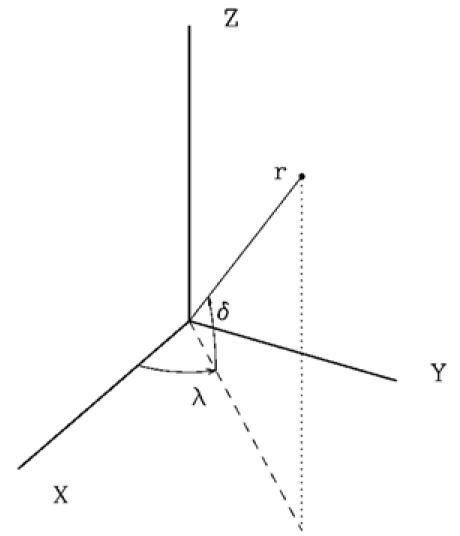
\includegraphics[width=0.7\textwidth]{figures/reference_frames/sphertocart_noomen2013basic.jpg}
\caption{Spherical position variables in an inertial Cartesian frame \citep{noomen2013basic}.}
\label{fig:sphertocart_noomen2013basic}
\end{figure}

\begin{align} \label{eq:transAngl}
\begin{split}
r = \sqrt{x^{2}+y^{2}+z^{2}}\\
\end{split}
&
\begin{split}
\sin \lambda &= \dfrac{y}{\sqrt{x^{2}+y^{2}}}\\
\cos \lambda &= \dfrac{x}{\sqrt{x^{2}+y^{2}}}\\
\end{split}
&
\begin{split}
\sin \delta &= \dfrac{z}{r}\\
\cos \delta &= \dfrac{\sqrt{x^{2}+y^{2}}}{r}
\end{split} 
\end{align} 

The corresponding auxiliary functions can then be described by \Cref{eq:auxFtransAngl} using the definitions provided in \Cref{eq:stateX,eq:state_derivativesX}.

\begin{align} \label{eq:auxFtransAngl}
\begin{split}
w_{4,1} &= x_{1}^{2}+x_{2}^{2} \\
w_{4,2} &= w_{4,1}+x_{3}^{2} \\
w_{4,3} &= r = \sqrt{w_{4,2}} \\
w_{4,4} &= \sqrt{w_{4,1}} \\
\end{split}
&
\begin{split}
w_{4,5} &= s\lambda = \dfrac{x_{2}}{w_{4,4}}\\
w_{4,6} &= c\lambda = \dfrac{x_{1}}{w_{4,4}} \\
\end{split}
&
\begin{split}
w_{4,7} &= s\delta = \dfrac{x_{3}}{w_{4,3}} \\
w_{4,8} &= c\delta = \dfrac{w_{4,4}}{w_{4,3}}\\
\end{split} 
\end{align} 


The latitude and longitude could be described using the position vector in the inertial frame, however the transformation from the body frame to the vertical frame is a function of the ground (underscore 'G') velocity in the rotational frame. Since the position and velocity in the inertial frame are known (current state), the ground velocity ($V_{G}$) can be written as a function of the inertial velocity ($V_{I}$). For this, the velocity components have to be transformed from the inertial frame to the vertical frame (which is the inverse of the first three transformations described in \Cref{eq:acc}). This transformation is shown in \Cref{eq:VItoVV} and was described in \cite{mooij1994motion}. Here, $c$ stands for cosine and $s$ stands for sine. This transformation also includes the rotational effect on the velocity due to the rotation of Mars.
 
 \begin{equation} \label{eq:VItoVV}
\mathbf{V_{V}} =  
 \begin{pmatrix}
V_{x_{V}}\\
V_{y_{V}}\\
V_{z_{V}}\\
\end{pmatrix}
=
\left[
\begin{matrix}
-c\lambda s\delta & -s\lambda s\delta & c\delta\\
-s\lambda & c\lambda & 0\\
-c\lambda c\delta & -s\lambda c\delta & -s\delta\\
\end{matrix}
\right]
\left\lbrace
\begin{pmatrix}
V_{x}\\
V_{y}\\
V_{z}\\
\end{pmatrix}
-
\begin{pmatrix}
0 \\
0 \\
\Omega_{M} \\
\end{pmatrix}
\times
\begin{pmatrix}
x \\
y \\
z \\
\end{pmatrix}
\right\rbrace
 \end{equation}
 
The ground velocity can now be computed as the norm of the vertical velocity vector as shown by \Cref{eq:VG}. The transformation matrices disappear because the norm of a transformation matrix is simply 1, which means that $V_{G}=V_{V}=V_{R}$.

\begin{equation} \label{eq:VG}
V_{G} = \| \mathbf{V_{V}} \| = 
\left\Vert
\begin{pmatrix}
V_{x}\\
V_{y}\\
V_{z}\\
\end{pmatrix}
-
\begin{pmatrix}
0 \\
0 \\
\Omega_{M} \\
\end{pmatrix}
\times
\begin{pmatrix}
x \\
y \\
z \\
\end{pmatrix}
\right\Vert 
\end{equation}

\Cref{eq:VG} can be rewritten as \Cref{eq:xfifteen}.

\begin{equation}\label{eq:xfifteen}
V_{G} = \sqrt{\left(V_{x}+\Omega_{M}y\right)^{2}+\left(V_{y}-\Omega_{M}x\right)^{2}+V_{z}^{2}} 
\end{equation}

The corresponding auxiliary functions are provided in \Cref{eq:velocityAuxF}.

\begin{align} \label{eq:velocityAuxF}
\begin{split}
w_{4,9} &= V_{x}+\Omega_{M}y = x_{4}+\Omega_{M}x_{2} \\
w_{4,10} &= V_{y}-\Omega_{M}x = x_{5}-\Omega_{M}x_{1} \\
\end{split}
&
\begin{split}
w_{4,11} &= w_{4,9}^{2}+w_{4,10}^{2}+x_{6}^{2} \\
w_{4,12} &= V_{G}=\sqrt{w_{4,11}} \\
\end{split} 
\end{align} 

%\sqrt{V_{I}^{2}+\Omega_{M}^{2}\left(x^{2}+y^{2}\right)+2\Omega_{M}\left(V_{x}y-V_{y}x\right)} \quad \text{where} \quad V_{I}=\sqrt{V_{x}^{2}+V_{y}^{2}+V_{z}^{2}} \\
 
The spherical velocity angles can now be derifed from \Cref{fig:vertical_spherical_mooij1994motion} as described by \Cref{eq:velAngl}. These were also provided by \cite{mooij1994motion}. 

 \begin{figure}[!ht]
\centering
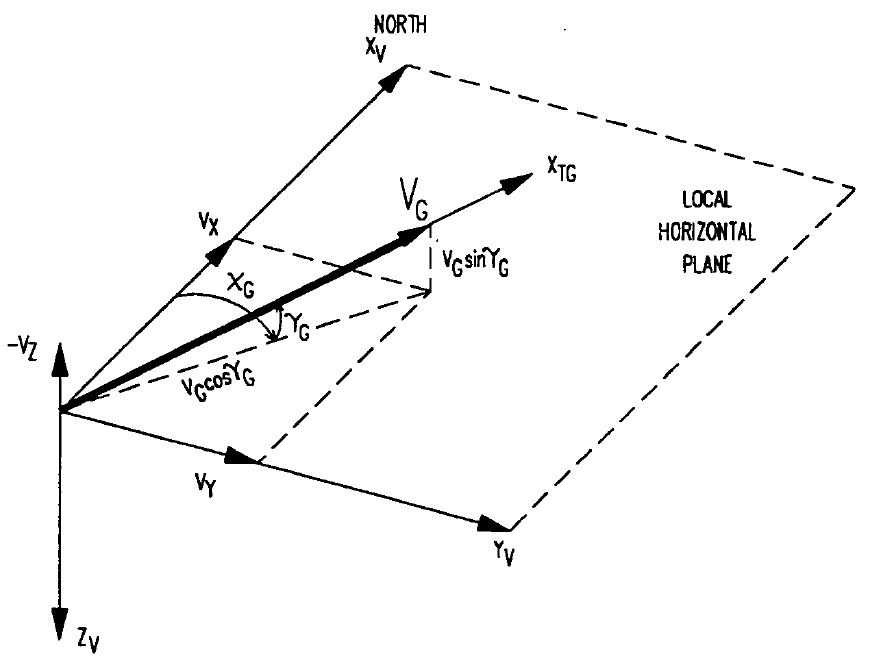
\includegraphics[width=0.7\textwidth]{figures/reference_frames/vertical_spherical_mooij1994motion.jpg}
\caption{Spherical velocity variables in a vertical Cartesian frame \citep{mooij1994motion}.}
\label{fig:vertical_spherical_mooij1994motion}
\end{figure}



\begin{align} \label{eq:velAngl}
\begin{split}
\sin \chi_{G} &= \dfrac{V_{y_{V}}}{\sqrt{V_{x_{V}}^{2}+V_{y_{V}}^{2}}} \\
\cos \chi_{G} &= \dfrac{V_{x_{V}}}{\sqrt{V_{x_{V}}^{2}+V_{y_{V}}^{2}}} \\
\end{split}
&
\begin{split}
\sin \gamma_{G} &= \dfrac{-V_{z_{V}}}{V_{G}}\\
\cos \gamma_{G} &= \dfrac{\sqrt{V_{x_{V}}^{2}+V_{y_{V}}^{2}}}{V_{G}}\\
\end{split} 
\end{align} 


Here, $V_{x_{V}}$, $V_{y_{V}}$ and $V_{z_{V}}$ are the velocities in the vertical frame. Expressions for these variables can be obtained by rewriting \Cref{eq:VItoVV}. This then results in \Cref{eq:VV}.


\begin{equation} \label{eq:VV}
\begin{split}
V_{x_{V}} & = -\left(V_{x}+\Omega_{M}y\right) s \delta c\lambda - \left(V_{y}-\Omega_{M}x\right) s\delta s\lambda+V_{z}c\delta \\
V_{y_{V}} & = \left(V_{y}-\Omega_{M}x\right) c\lambda - \left(V_{x}+\Omega_{M} y \right) s\lambda \\
V_{z_{V}} & = -\left(V_{x}+\Omega_{M}y\right)c\delta c\lambda-\left(V_{y}-\Omega_{M}x\right) c\delta s\lambda - V_{z} s\delta \\
\end{split}
\end{equation}

The combined auxiliary functions for \Cref{eq:velAngl,eq:VV} are described in \Cref{eq:velocityAuxF}.

\begin{align} \label{eq:VV}
\begin{split}
w_{4,13} &= -c\lambda s\delta  = -w_{4,6}w_{4,7} \\
w_{4,14} &= -s\delta s\lambda = -w_{4,7}w_{4,5} \\
w_{4,15} &= -c\delta c\lambda = -w_{4,8}w_{4,6} \\
w_{4,16} &= -c\delta s\lambda = w_{4,8}w_{4,5} \\
\end{split}
&
\begin{split}
w_{4,17} &= V_{x_{V}} = x_{6}w_{4,8}+w_{4,9}w_{4,13}+w_{4,10}w_{4,14} \\
w_{4,18} &= V_{y_{V}} = w_{4,10}w_{4,6}-w_{4,9}w_{4,5} \\
w_{4,19} &= V_{z_{V}} = w_{4,9}w_{4,15}-x_{6}w_{4,7}+w_{4,10}w_{4,16} \\
w_{4,20} &= V_{x_{V}}^{2}+V_{y_{V}}^{2} = w_{4,17}^{2}+w_{4,18}^{2} \\
w_{4,21} &= \sqrt{w_{4,20}} \\
\end{split}
&
\begin{split}
w_{4,22} &= s\chi_{G} = \dfrac{w_{4,18}}{w_{4,21}} \\
w_{4,23} &= c\chi_{G} = \dfrac{w_{4,17}}{w_{4,21}} \\
w_{4,24} &= s\gamma_{G} = -\dfrac{w_{4,19}}{w_{4,12}} \\
w_{4,25} &= c\gamma_{G} = \dfrac{w_{4,21}}{w_{4,12}} \\
\end{split}
\end{align}



 \subsubsection{Drag acceleration}
 \label{subsubsec:tsiDrag}
The drag acceleration is determined in the body frame by dividing the drag force ($D$) by the mass of the \ac{MAV} ($x_{7}$). The drag force itself is a function of the position and velocity. The equations associated with the drag function are described in \Cref{eq:drag} except for the $C_{D}$ equations. The polynomial coefficients for the density equation are provided in \Cref{tab:fitParametersDen} and are represented in \Cref{eq:drag} by $P_{\rho}$.

 \begin{equation} \label{eq:drag}
\begin{split}
h &= r-R_{MOLA} \\
D &= \frac{1}{2}\rho V_{G}^{2}SC_{D}\\
\rho &= e^{P_{\rho 10}h^{10}+P_{\rho 9}h^{9}+P_{\rho 8}h^{8}+P_{\rho 7}h^{7}+P_{\rho 6}h^{6}+P_{\rho 5}h^{5}+P_{\rho 4}h^{4}+P_{\rho 3}h^{3}+P_{\rho 2}h^{2}+P_{\rho 1}h+P_{\rho 0}} \\
\end{split}
\end{equation}

The numbering for the drag auxiliary functions start with 27 because it was added later on and because it used to be an auxiliary equation. The auxiliary functions for the density can then be described by \Cref{eq:dragAuxF}.

\begin{align} \label{eq:dragAuxF}
\begin{split}
w_{27,1} &= h = w_{4,3} - R_{MOLA} \\
w_{27,2} &= w_{27,1}^{2}\\
w_{27,3} &= w_{27,1}^{3}\\
w_{27,4} &= w_{27,1}^{4}\\
w_{27,5} &= w_{27,1}^{5}\\
w_{27,6} &= w_{27,1}^{6}\\
\end{split}
&
\begin{split}
w_{27,7} &= w_{27,1}^{7}\\
w_{27,8} &= w_{27,1}^{8}\\
w_{27,9} &= w_{27,1}^{9}\\
w_{27,10} &= w_{27,1}^{10}\\
w_{27,11} &= P_{\rho 10}w_{27,10}+P_{\rho 9}w_{27,9}+\dotsc +P_{\rho 1}w_{27,1}+P_{\rho 0}\\
w_{27,12} &= \rho = e^{w_{27,11}} \\
\end{split}
\end{align}

Since the drag coefficient is a function of Mach number as by \Cref{fig:dragcoeff_whitehead2004mars} and is not a continuous function, it has to be split into 6 different sections. Each section has a separate $C_{D}-M$ relation. Before these relations can be described, three additional expressions are required which are described in \Cref{eq:cd}.

 \begin{equation} \label{eq:cd}
\begin{split}
M &= \dfrac{V_{G}}{a} \\
a &= \sqrt{\gamma_{a}R_{a}^{*}T_{a}} \quad \text{where} \quad R_{a}^{*}=\dfrac{R_{a}}{M_{a}} \\
\end{split}
\end{equation}

Where the corresponding auxiliary functions can be described by \Cref{eq:cdAuxF}.

\begin{align} \label{eq:cdAuxF}
\begin{split}
w_{27,14} &= a = \sqrt{\gamma_{a}R_{a}^{*}w_{27,13}}  \\
w_{27,15} &= M = \dfrac{w_{4,12}}{w_{27,14}} \\
\end{split}
\end{align}

The conditional relations shown in \Cref{eq:cdCondC} describe the different equations that have to be used associated with the different sections of the drag coefficient plot. Here $P_{C_{D} number,section}$ are the polynomial fit coefficients as provided in \Cref{tab:dragCoeffPara}.

\begin{equation}\label{eq:cdCondC}
C_{D}=\begin{cases}
0.2, & \text{for } 0\leq M < 0.5\\
P_{C_{D} 1,2}M+P_{C_{D} 0,2}, &  \text{for } 0.5\leq M < 1 \\
P_{C_{D} 1,3}M+P_{C_{D} 0,3}, &  \text{for } 1\leq M < 1.3 \\
P_{C_{D} 1,4}M+P_{C_{D} 0,4}, &  \text{for } 1.3\leq M < 2.5 \\
P_{C_{D} 1,5}M+P_{C_{D} 0,5}, &  \text{for } 2.5\leq M < 4 \\
0.3, &  \text{for } M \geq 4 
\end{cases}\\
\end{equation}

In this case, the auxiliary functions for $C_{D} \left( = w_{27,16}\right)$ is any of the conditional relations depending on $M \left( = w_{27,15}\right)$.

This only leaves the temperature $T_{a} \left(= w_{27,13}\right)$ , which is a function of the altitude $h \left(= w_{27,1} \right) $ in km,\ac{MOLA}. But as described in \Cref{subsec:atmofuncfit}, this parameter is split into different sections as well. The equations per section for the temperature is provided in \Cref{eq:tempCondAuxC}. Here $P_{T number,section}$ are the polynomial fit coefficients as provided in \Cref{tab:fitParameters}.

\begin{equation}\label{eq:tempCondAuxC}
T_{a}=\begin{cases}
P_{T 1,1}h+P_{T 0,1}, & \text{for } -0.6 \leq h < 5.04  \\
P_{T 3,2}h^{3}+P_{T 2,2}h^{2}+P_{T 1,2}h+P_{T 0,2}, &  \text{for } 5.04 \leq h < 35.53   \\
P_{T 6,3}h^{6}+P_{T 5,3}h^{5}+P_{T 4,3}h^{4}+P_{T 3,3}h^{3}+ \dotsc \\
\qquad\ \ \dotsc +P_{T 2,3}h^{2}+P_{T 1,3}h+P_{T 0,3}, &  \text{for } 35.53 \leq h < 75.07   \\
P_{T 8,4}h^{8}+P_{T 7,4}h^{7}+P_{T 6,4}h^{6}+P_{T 5,4}h^{5}+ \dotsc \\
\qquad\ \ \dotsc+P_{T 4,4}h^{4}+P_{T 3,4}h^{3}+P_{T 2,4}h^{2}+P_{T 1,4}h+P_{T 0,4}, &  \text{for } 75.07 \leq h < 170.05   \\
136.5, &  \text{for }  h \geq 170.05   
\end{cases}
\end{equation}

For both the conditional parameters $C_{D}$ and $T_{a}$  the required section has to be determined before the evaluation of the equations.

The drag can now also be described as an auxiliary function as shown by \Cref{eq:dragAuxF}.

\begin{align} \label{eq:dragAuxF}
\begin{split}
w_{27,17} &= V_{G}^{2} =  w_{4,12}^{2} \\
w_{27,18} &= V_{G}^{2}C_{D} = w_{27,17}w_{27,16} \\
w_{27,19} &= D = \frac{1}{2} S w_{27,18}w_{27,12} \\
\end{split}
\end{align}



\subsubsection{Thrust acceleration}
\label{subsubsec:tsiThrust}
The only acceleration component still missing is the thrust acceleration. To be able to write the auxiliary functions for the thrust, \Cref{eq:acc} first has to be rewritten such that all the transformations are gathered into two transformation matrices (see \Cref{eq:accAux}). The transformation matrices are described by \Cref{eq:BPtrans,eq:IBtrans} for $\mathbb{T}_{\mathbf{BP}}$ and $\mathbb{T}_{\mathbf{IB}}$ respectively.

\begin{equation} \label{eq:accAux}
\begin{pmatrix}
x'_{4}\\
x'_{5}\\
x'_{6}\\
\end{pmatrix}
=
\begin{pmatrix}
-\mu_{M}\dfrac{x_{1}}{x_{9}}\\
-\mu_{M}\dfrac{x_{2}}{x_{9}}\\
-\mu_{M}\dfrac{x_{3}}{x_{9}}\\
\end{pmatrix}+
\mathbb{T}_{\mathbf{IB}}\left[
\begin{pmatrix}
-\dfrac{w_{27,19}}{x_{7}}\\
0\\
0\\
\end{pmatrix}
+ 
\mathbb{T}_{\mathbf{BP}}
\begin{pmatrix}
\dfrac{T}{x_{7}}\\
0\\
0\\
\end{pmatrix}
\right]
\end{equation}


\begin{equation} \label{eq:BPtrans}
\mathbb{T}_{\mathbf{BP}}=
\begin{bmatrix}
c\psi_{T}c\epsilon_{T} & -s\psi_{T} & c\psi_{T}s\epsilon_{T}\\
s\psi_{T}c\epsilon_{T} & c\psi_{T} & s\psi_{T}s\epsilon_{T}\\
-s\epsilon_{T} & 0 & c\epsilon_{T}\\
\end{bmatrix}
\end{equation}

\begin{equation} \label{eq:IBtrans}
\mathbb{T}_{\mathbf{IB}}=
\left[
\begin{matrix}
c\lambda\left(-s\delta c\chi c\gamma +c\delta s\gamma \right)-s\lambda s\chi c\gamma  & c\lambda s\delta s\chi -s\lambda c\chi & c\lambda\left(-s\delta c\chi s\gamma -c\delta c\gamma \right)-s\lambda s\chi s\gamma \\
s\lambda\left(-s\delta c\chi c\gamma +c\delta s\gamma \right)+c\lambda s\chi c\gamma & s\lambda s\delta s\chi +c\lambda c\chi & s\lambda\left(-s\delta c\chi s\gamma -c\delta c\gamma \right)+c\lambda s\chi s\gamma \\
c\delta c\chi c\gamma +s\delta s\gamma &  -c\delta s\chi &  c\delta c\chi s\gamma -s\delta c\gamma \\
\end{matrix}
\right]\\
\end{equation}



%\end{matrix}  \right.
%\\
%\begin{matrix}
%c\lambda s\delta s\chi -s\lambda c\chi\\
%s\lambda s\delta s\chi +c\lambda c\chi \\
% -c\delta s\chi \\
%\end{matrix}
%\\
%\left.
%\begin{matrix}
%c\lambda\left(-s\delta c\chi s\gamma -c\delta c\gamma \right)-s\lambda s\chi s\gamma\\
%s\lambda\left(-s\delta c\chi s\gamma -c\delta c\gamma \right)+c\lambda s\chi s\gamma \\
%c\delta c\chi s\gamma -s\delta c\gamma\\
%=
%\left[
%\begin{matrix}
%c\left(x_{10}+x_{11}\right)\left(-sx_{12} cx_{13} cx_{14} +cx_{12} sx_{14} \right)-s\left(x_{10}+x_{11}\right) sx_{13} cx_{14}    \\
%s\left(x_{10}+x_{11}\right)\left(-sx_{12} cx_{13} cx_{14} +cx_{12} sx_{14} \right)+c\left(x_{10}+x_{11}\right) sx_{13} cx_{14}    \\
%cx_{12} cx_{13} cx_{14} +sx_{12} sx_{14}   \\
%\end{matrix} \right.
%\\
%\begin{matrix}
%c\left(x_{10}+x_{11}\right) sx_{12} sx_{13} -s\left(x_{10}+x_{11}\right) cx_{13} \\
%s\left(x_{10}+x_{11}\right) sx_{12} sx_{13} +c\left(x_{10}+x_{11}\right) cx_{13} \\
%-cx_{12} sx_{13} \\
%\end{matrix}
%\\
%\left.
%\begin{matrix}
%c\left(x_{10}+x_{11}\right)\left(-sx_{12} cx_{13} sx_{14} -cx_{12} cx_{14} \right)-s\left(x_{10}+x_{11}\right) sx_{13} sx_{14} \\
%s\left(x_{10}+x_{11}\right)\left(-sx_{12} cx_{13} sx_{14} -cx_{12} cx_{14} \right)+c\left(x_{10}+x_{11}\right) sx_{13} sx_{14} \\
% cx_{12} cx_{13} sx_{14} -sx_{12} cx_{14} \\
%\end{matrix}
%\right]\\

The thrust accelerations in the x-, y- and z-directions (in the body frame) can now be found by rewriting the last part of \Cref{eq:accAux} to \Cref{eq:aTB} using \Cref{eq:BPtrans}.

\begin{equation} \label{eq:aTB}
\mathbb{T}_{\mathbf{BP}}
\begin{pmatrix}
\dfrac{T}{x_{7}}\\
0\\
0\\
\end{pmatrix}
=
\begin{pmatrix}
\dfrac{T}{x_{7}}c\psi_{T}c\epsilon_{T}\\
\dfrac{T}{x_{7}}s\psi_{T}c\epsilon_{T}\\
-\dfrac{T}{x_{7}}s\epsilon_{T}\\
\end{pmatrix}
\end{equation}

%=
%\begin{pmatrix}
%a_{T_{B},x}\\
%a_{T_{B},y}\\
%a_{T_{B},z}\\
%\end{pmatrix}

\Cref{eq:aTB} can be expressed as a collection of auxiliary functions as well. These are described in \Cref{eq:aTBAuxF}.

\begin{align} \label{eq:aTBAuxF}
\begin{split}
w_{4,26} &= \cos \psi_{T} \\
w_{4,27} &= \cos \epsilon_{T} \\
w_{4,28} &= \sin \psi_{T} \\
w_{4,29} &= \sin \epsilon_{T} \\
w_{4,30} &= c\psi_{T} c\epsilon_{T} = w_{4,26}w_{4,27} \\
w_{4,31} &= c\epsilon_{T} s\psi_{T} = w_{4,27}w_{4,28} \\
w_{4,32} &= \dfrac{1}{x_{7}}\\
\end{split}
&
\begin{split}
w_{4,33} &= \dfrac{T}{x_{7}} = T w_{4,32}\\
w_{4,34} &= \dfrac{T}{x_{7}} c\epsilon_{T} c\psi_{T} = w_{4,33}w_{4,30} \\
w_{4,37} &= \dfrac{T}{x_{7}}c\epsilon_{T} s\psi_{T} = w_{4,33}w_{4,31} \\
w_{4,38} &= \dfrac{T}{x_{7}} s\epsilon_{T} = w_{4,33}w_{4,29} \\
\end{split}
\end{align}


The thrust accelerations are now written in the body frame, which means that they can be combined with the drag acceleration in the body frame. This is done in \Cref{eq:DandTBody}. Here, $w_{4,35}$ represents the drag acceleration in the body frame and $w_{4,36}$ is the total acceleration in the x-direction in the body frame caused by both the drag and the thrust.

%However, since both the thrust and drag accelerations include auxiliary equations ($x_{7}$ and $x_{27}$) the total acceleration in the body frame in the different directions have to be expressed as auxiliary functions. Each auxiliary function replaces one algebraic operation such as multiplication, division, power, exponential and trigonometric functions. Auxiliary functions will be represented by $w_{n,m}$ as per convention introduced by \cite{scott2008high}. Here $n$ stands for the associating derivative and $m$ represents the number of the auxiliary function for that particular derivative. These auxiliary functions will be used to write the different parameters into recurrence relations.

\begin{equation} \label{eq:DandTBody}
\begin{pmatrix}
-\dfrac{x_{27}}{x_{7}}\\
0\\
0\\
\end{pmatrix}
+
\begin{pmatrix}
w_{4,34}\\
w_{4,37}\\
-w_{4,38}\\
\end{pmatrix}
=
\begin{pmatrix}
w_{4,34}-w_{4,35}\\
w_{4,37}\\
-w_{4,38}\\
\end{pmatrix}
=
\begin{pmatrix}
w_{4,36}\\
w_{4,37}\\
-w_{4,38}\\
\end{pmatrix}
\end{equation}

\subsubsection{All accelerations combined}
\label{subsubsec:allAcc}
At this point the gravity accelerations are known in the inertial frame and the drag and thrust accelerations in the body frame. In order to get the final acceleration vector in the inertial frame, the drag and thrust accelerations have to be transformed from the body frame to the inertial frame using $\mathbb{T}_{\mathbf{IB}}$ resulting in \Cref{eq:DandTInertial}.



\begin{equation} \label{eq:DandTInertial}
\mathbb{T}_{\mathbf{IB}}
\begin{pmatrix}
w_{4,36}\\
w_{4,37}\\
-w_{4,38}\\
\end{pmatrix}
=
\left(
\begin{matrix}
w_{4,36}\left( c\lambda\left(-s\delta c\chi c\gamma +c\delta s\gamma \right)-s\lambda s\chi c\gamma \right)  +w_{4,37} \left( c\lambda s\delta s\chi -s\lambda c\chi\right)  -w_{4,38} \left( c\lambda\left(-s\delta c\chi s\gamma -c\delta c\gamma \right)-s\lambda s\chi s\gamma \right) \\
w_{4,36} \left( s\lambda\left(-s\delta c\chi c\gamma +c\delta s\gamma \right)+c\lambda s\chi c\gamma \right) +w_{4,37} \left( s\lambda s\delta s\chi +c\lambda c\chi \right)  -w_{4,38} \left( s\lambda\left(-s\delta c\chi s\gamma -c\delta c\gamma \right)+c\lambda s\chi s\gamma \right) \\
w_{4,36} \left( c\delta c\chi c\gamma +s\delta s\gamma\right) + w_{4,37} \left(  -c\delta s\chi \right) -w_{4,38} \left(  c\delta c\chi s\gamma -s\delta c\gamma \right) \\
\end{matrix}
\right)\\
\end{equation}

%\begin{pmatrix}
%a_{T,D_{I},x}\\
%a_{T_{I},y}\\
%a_{T_{I},z}\\
%\end{pmatrix}
%=
%\mathbb{T}_{\mathbf{IB}}
%\begin{pmatrix}
%a_{T,D_{B},x}\\
%a_{T_{B},y}\\
%a_{T_{B},z}\\
%\end{pmatrix}=
%\left(
%\begin{matrix}
%w_{4,2} \left( c\left(x_{10}+x_{11}\right)\left(-sx_{12} cx_{13} cx_{14} +cx_{12} sx_{14} \right)-s\left(x_{10}+x_{11}\right) sx_{13} cx_{14} \right)  + \dots  \\
%w_{4,2} \left( s\left(x_{10}+x_{11}\right)\left(-sx_{12} cx_{13} cx_{14} +cx_{12} sx_{14} \right)+c\left(x_{10}+x_{11}\right) sx_{13} cx_{14}  \right)  + \dots \\
%w_{4,2} \left(cx_{12} cx_{13} cx_{14} +sx_{12} sx_{14}  \right)  - \dots \\
%\end{matrix} \right.
%\\
%\begin{matrix}
%\dotsc  w_{4,33} \left( c\left(x_{10}+x_{11}\right) sx_{12} sx_{13} -s\left(x_{10}+x_{11}\right) cx_{13}\right)  - \dots \\
%\dotsc  w_{4,33} \left( s\left(x_{10}+x_{11}\right) sx_{12} sx_{13} +c\left(x_{10}+x_{11}\right) cx_{13} \right)  - \dots \\
%\dotsc  w_{4,33} cx_{12} sx_{13} - \dots \\
%\end{matrix}
%\\
%\left.
%\begin{matrix}
%\dotsc w_{4,34} \left( c\left(x_{10}+x_{11}\right)\left(-sx_{12} cx_{13} sx_{14} -cx_{12} cx_{14} \right)-s\left(x_{10}+x_{11}\right) sx_{13} sx_{14} \right) \\
%\dotsc w_{4,34} \left(s\left(x_{10}+x_{11}\right)\left(-sx_{12} cx_{13} sx_{14} -cx_{12} cx_{14} \right)+c\left(x_{10}+x_{11}\right) sx_{13} sx_{14} \right) \\
%\dotsc w_{4,34} \left( cx_{12} cx_{13} sx_{14} -sx_{12} cx_{14} \right) \\
%\end{matrix}
%\right)\\

Now including the gravity components as well, the (lengthy) expressions for $x'_{4}$, $x'_{5}$ and $x'_{6}$ become \Cref{eq:u4Com,eq:u5Com,eq:u6Com} respectively.

\begin{equation} \label{eq:u4Com}
\begin{split}
x'_{4}= -\mu_{M}\dfrac{x_{1}}{x_{9}}&+w_{4,36}\left( c\lambda\left(-s\delta c\chi c\gamma +c\delta s\gamma \right)-s\lambda s\chi c\gamma \right)+ \dots \\
& \dotsc  w_{4,37} \left( c\lambda s\delta s\chi -s\lambda c\chi\right)-\dots \\
& \dotsc w_{4,38} \left( c\lambda\left(-s\delta c\chi s\gamma -c\delta c\gamma \right)-s\lambda s\chi s\gamma \right)
\end{split}
\end{equation}

\begin{equation} \label{eq:u5Com}
\begin{split}
x'_{5}= -\mu_{M}\dfrac{x_{2}}{x_{9}}&+w_{4,36} \left( s\lambda\left(-s\delta c\chi c\gamma +c\delta s\gamma \right)+c\lambda s\chi c\gamma \right)+ \dots \\
& \dotsc w_{4,37} \left( s\lambda s\delta s\chi +c\lambda c\chi \right) - \dots \\
& \dotsc w_{4,38} \left( s\lambda\left(-s\delta c\chi s\gamma -c\delta c\gamma \right)+c\lambda s\chi s\gamma \right)
\end{split}
\end{equation} 

\begin{equation} \label{eq:u6Com}
\begin{split}
x'_{6}= -\mu_{M}\dfrac{x_{3}}{x_{9}}&+w_{4,36} \left( c\delta c\chi c\gamma +s\delta s\gamma\right) +  w_{4,37} \left(  -c\delta s\chi \right)  -w_{4,38} \left(  c\delta c\chi s\gamma -s\delta c\gamma \right)
\end{split}
\end{equation}

%\begin{equation} \label{eq:u4Com}
%\begin{split}
%x'_{4}= -\mu_{M}\dfrac{x_{1}}{x_{9}}&+w_{4,2} \left( c\left(x_{10}+x_{11}\right)\left(-sx_{12} cx_{13} cx_{14} +cx_{12} sx_{14} \right)-s\left(x_{10}+x_{11}\right) sx_{13} cx_{14} \right)+ \dots \\
%& \dotsc  w_{4,33} \left( c\left(x_{10}+x_{11}\right) sx_{12} sx_{13} -s\left(x_{10}+x_{11}\right) cx_{13}\right)-\dots \\
%& \dotsc w_{4,34} \left( c\left(x_{10}+x_{11}\right)\left(-sx_{12} cx_{13} sx_{14} -cx_{12} cx_{14} \right)-s\left(x_{10}+x_{11}\right) sx_{13} sx_{14} \right)
%\end{split}
%\end{equation}
%
%\begin{equation} \label{eq:u5Com}
%\begin{split}
%x'_{5}= -\mu_{M}\dfrac{x_{2}}{x_{9}}&+w_{4,2} \left( s\left(x_{10}+x_{11}\right)\left(-sx_{12} cx_{13} cx_{14} +cx_{12} sx_{14} \right)+c\left(x_{10}+x_{11}\right) sx_{13} cx_{14}  \right)+ \dots \\
%& \dotsc w_{4,33} \left( s\left(x_{10}+x_{11}\right) sx_{12} sx_{13} +c\left(x_{10}+x_{11}\right) cx_{13} \right)- \dots \\
%& \dotsc w_{4,34} \left(s\left(x_{10}+x_{11}\right)\left(-sx_{12} cx_{13} sx_{14} -cx_{12} cx_{14} \right)+c\left(x_{10}+x_{11}\right) sx_{13} sx_{14} \right)
%\end{split}
%\end{equation} 
%
%\begin{equation} \label{eq:u6Com}
%\begin{split}
%x'_{6}= -\mu_{M}\dfrac{x_{3}}{x_{9}}&+w_{4,2} \left(cx_{12} cx_{13} cx_{14} +sx_{12} sx_{14}  \right)  - w_{4,33}cx_{12} sx_{13}  -w_{4,34} \left( cx_{12} cx_{13} sx_{14} -sx_{12} cx_{14} \right)
%\end{split}
%\end{equation}

These equations now have to be written as a collection of auxiliary functions for the x-, y- and z-direction in the inertial frame. The gravitational acceleration can be written as the vector shown by \Cref{eq:gravAuxF}.

\begin{equation} \label{eq:gravAuxF}
\mathbf{a_{g}} =
\begin{pmatrix}
-\mu_{M}\dfrac{x_{1}}{x_{9}} \\
-\mu_{M}\dfrac{x_{2}}{x_{9}} \\
-\mu_{M}\dfrac{x_{3}}{x_{9}} \\
\end{pmatrix}
= 
\begin{pmatrix}
w_{4,39} \\
w_{5,1} \\
w_{6,1} \\
\end{pmatrix}
\end{equation}

The auxiliary derivatives ($u = x'$) can now be defined as the collection of auxiliary functions that describe the different transformations for $u_{4}, u_{5} and u_{6}$. These are shown in \Cref{eq:u4AuxF,eq:u5AuxF,eq:u6AuxF} respectively. 

\begin{align} \label{eq:u4AuxF}
\begin{split}
w_{4,40} &= -s\delta c\chi_{G} = -w_{4,7}w_{4,23} \\
w_{4,41} &= c\delta	s\gamma_{G} = w_{4,8}w_{4,24}\\
w_{4,42} &= -s\lambda s\chi_{G} = -w_{4,5}w_{4,22}\\
w_{4,43} &= -s\lambda c\chi_{G} = -w_{4,5}w_{4,23} \\
w_{4,44} &= -c\delta c\gamma_{G} = -w_{4,8}w_{4,25} \\
w_{4,45} &= w_{4,40} c\gamma_{G} = w_{4,40}w_{4,25} \\
\end{split}
&
\begin{split}
w_{4,46} &= w_{4,42} c\gamma_{G} = w_{4,42}w_{4,25} \\
w_{4,47} &= -w_{4,13} s\chi_{G} = -w_{4,13}w_{4,22} \\
w_{4,48} &= w_{4,40} s\gamma_{G} = w_{4,40}w_{4,24} \\
w_{4,49} &= w_{4,42} s\gamma_{G} = w_{4,42}w_{4,24} \\
w_{4,50} &= c\lambda \left(w_{4,45}+w_{4,41} \right) + w_{4,46} = 
w_{4,6}\left(w_{4,45}+w_{4,41} \right) + w_{4,46} \\
w_{4,51} &= c\lambda \left(w_{4,48}+w_{4,44} \right) + w_{4,49} =
w_{4,6}\left(w_{4,48}+w_{4,44} \right) + w_{4,49} \\
w_{4,52} &= w_{4,39} +w_{4,36}w_{4,50}+w_{4,37}\left(w_{4,47}+w_{4,43}\right)-w_{4,38}w_{4,51} \\
u_{4} &= w_{4,52} \\
\end{split}
\end{align}

\begin{align} \label{eq:u5AuxF}
\begin{split}
w_{5,2} &= c\lambda s\chi_{G} = w_{4,6}w_{4,22} \\
w_{5,3} &= s\lambda \left(w_{4,45}+w_{4,41}\right)+w_{5,2} c\gamma_{G} = w_{4,5} \left(w_{4,45}+w_{4,41}\right) +w_{5,2} w_{4,25} \\
w_{5,4} &= -w_{4,14} s\chi_{G}+c\lambda c\chi_{G} = -w_{4,14}w_{4,22}+w_{4,6}w_{4,23} \\
w_{5,5} &= s\lambda \left(w_{4,48}+w_{4,44}\right) + w_{5,2} s\gamma_{G} = w_{4,5} \left(w_{4,48}+w_{4,44}\right)+w_{5,2}w_{4,24} \\
w_{5,6} &= w_{5,1} + w_{4,36}w_{5,3}+w_{4,37}w_{5,4}-w_{4,38}w_{5,5} \\
u_{5} &= w_{5,6} \\
\end{split}
\end{align}

\begin{align} \label{eq:u6AuxF}
\begin{split}
w_{6,2} &= s\delta s\gamma_{G} = w_{4,7}w_{4,24} \\
w_{6,3} &= c\delta s\chi_{G} = w_{4,8}w_{4,22} \\
w_{6,4} &= -s\delta c\gamma_{G} = -w_{4,7}w_{4,25} \\
\end{split}
&
\begin{split}
w_{6,5} &= -w_{4,44} c\chi_{G} +w_{6,2} = -w_{4,44}w_{4,23}+w_{6,2} \\
w_{6,6} &= w_{4,41} c\chi_{G} + w_{6,4} = w_{4,41}w_{4,23}+w_{6,4} \\
w_{6,7} &= w_{6,1} + w_{4,36}w_{6,5}-w_{4,37}w_{6,3}-w_{4,38}w_{6,6} \\
u_{6} &= w_{6,7} \\
\end{split}
\end{align}

Also, because auxiliary equations were used for the gravitational acceleration. The corresponding auxiliary derivatives can be written as a collection of auxiliary functions as shown in \Cref{eq:u8u9AuxF}.

\begin{align} \label{eq:u8u9AuxF}
\begin{split}
w_{8,1} &= x_{1}x_{4} \\
w_{8,2} &= x_{2}x_{5} \\
w_{8,3} &= x_{3}x_{6} \\
u_{8} &= 2\left(w_{8,1}+w_{8,2}+w_{8,3}\right) \\ 
\end{split}
&
\begin{split}
w_{9,0} &= x_{9}u_{8} \\
w_{9,1} &= \dfrac{w_{9,0}}{x_{8}} \\
u_{9} &= 1.5 w_{9,1} \\
\end{split}
\end{align}

Then the equations in \Cref{eq:restAuxD} complete the whole set of auxiliary derivatives.

\begin{align} \label{eq:restAuxD}
\begin{split}
u_{1} &= x_{4} \\
u_{2} &= x_{5} \\
\end{split}
&
\begin{split}
u_{3} &= x_{6} \\
u_{7} &= -\dfrac{T}{g_{0}I_{sp}} \\
\end{split}
\end{align}

 
\subsection{Cartesian equations, second case}
\label{subsec:careq2}
The second case (based on a method described by \citep{bergsma2015application}) is similar to the first case in terms of set-up of the dynamic equations, the gravitational acceleration, and the drag and thrust accelerations in the body frame. The only difference lies in the formulation of $\mathbb{T}_{\mathbf{IB}}$. Instead of using Euler angles and rotation transformation matrices, $\mathbb{T}_{\mathbf{IB}}$ can be set-up as one single matrix performing a direct transformation. This matrix is described in \Cref{eq:transMatCoef}, where $C$ stands for transformation matrix coefficient. 

\begin{equation} \label{eq:transMatCoef}
\mathbb{T}_{\mathbf{IB}} = 
\left[
\begin{matrix}
C_{1} & C_{4} & C_{7} \\
C_{2} & C_{5} & C_{8} \\
C_{3} & C_{6} & C_{9} \\
\end{matrix}
\right]
\end{equation}

\nomenclature[Ra1]{$C$}{Transformation matrix coefficient \nomunit{-}}

As was seen in \Cref{subsubsec:tsiTransAngl} the rotation from the vertical to the inertial frame is purely a function of the radius in the inertial frame ($\mathbf{r}$ or $\mathbf{r_{I}}$) Also, the transformation from the body frame to the vertical frame was purely a function of the ground velocity in the vertical frame ($\mathbf{V_{V}}$ or $\mathbf{V_{G_{V}}}$). Therefore, if this transformation is to be done in one transformation, the ground velocity in the inertial frame is required ($\mathbf{V_{G_{I}}}$), because it would transform directly to the inertial frame. This means that the coefficients in \Cref{eq:transMatCoef} will have to be a function of $\mathbf{r_{I}}$ and $\mathbf{V_{G_{I}}}$, where $\mathbf{V_{G_{I}}}$ is given by \Cref{eq:VGI}.

\begin{equation} \label{eq:VGI}
\mathbf{V_{G_{I}}} = 
\begin{pmatrix}
V_{x}\\
V_{y}\\
V_{z}\\
\end{pmatrix}
-
\begin{pmatrix}
0 \\
0 \\
\Omega_{M} \\
\end{pmatrix}
\times
\begin{pmatrix}
x \\
y \\
z \\
\end{pmatrix}=
\begin{pmatrix}
V_{x}+\Omega_{M}y \\
V_{y}-\Omega_{M}x \\
V_{z} \\
\end{pmatrix}
\end{equation}

\subsubsection{Body frame unit vectors}
So when looking from the inertial frame, there are two state vectors: position and ground velocity. The state changes part due to the accelerations in the body frame $\mathbf{a_{B}}$, which is a vector comprised of the drag and thrust accelerations. This vector has the same length and direction in the body frame and the inertial frame. Also, any vector is simply a multiplication of the corresponding unit vector. The same holds for the velocity, which means that because the velocity in the body frame is defined through the x-axis of that frame, the unit vector of the ground velocity can be described as the unit vector in the x-direction $\mathbf{\hat{i}}$ as shown by \Cref{eq:iHat}.

\begin{equation} \label{eq:iHat}
\mathbf{\hat{i}} = \dfrac{\mathbf{V_{G_{I}}}}{\| \mathbf{V_{G_{I}}}\|}
\end{equation}

\nomenclature[Ra3]{$\mathbf{\hat{i}}$}{Unit vector in x-direction \nomunit{-}}
\nomenclature[Ra3]{$\mathbf{\hat{j}}$}{Unit vector in y-direction \nomunit{-}}
\nomenclature[Ra2]{$\mathbf{\hat{h}}$}{Unit vector in z-direction \nomunit{-}}


This unit vector is also shown in \Cref{fig:cartesian_transformation_mooij1994motion}.

 \begin{figure}[!ht]
\centering
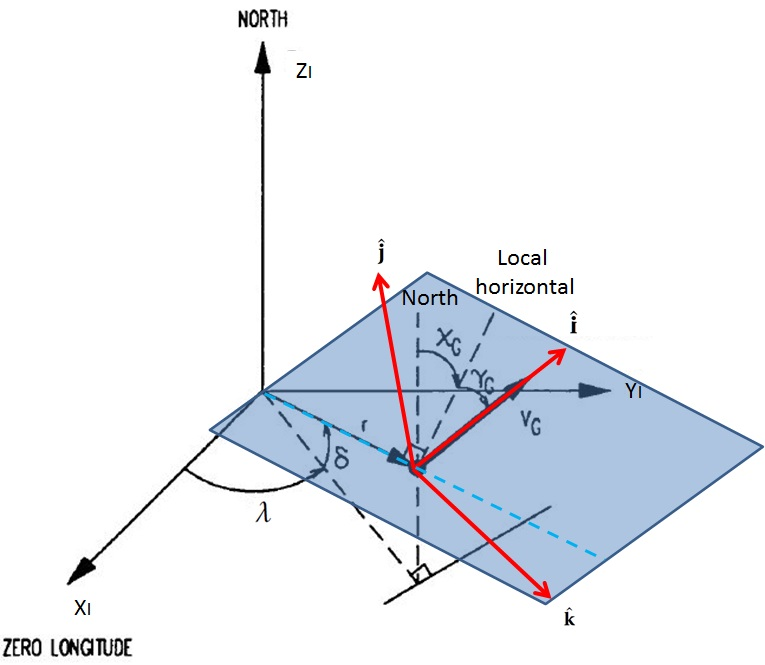
\includegraphics[width=0.7\textwidth]{figures/reference_frames/cartesian_transformation_mooij1994motion.jpg}
\caption{Definition of the body frame unit vectors based on the radius and ground velocity expressed in the inertial frame. \citep{mooij1994motion}}
\label{fig:cartesian_transformation_mooij1994motion}
\end{figure}

In \Cref{fig:cartesian_transformation_mooij1994motion} it can be seen that the z-axis unit vector $\mathbf{\hat{k}}$ is defined in the same plane as $\mathbf{\hat{i}}$, $\mathbf{V_{G_{I}}}$ and $\mathbf{r_{I}}$ perpendicular to $\mathbf{\hat{i}}$. As a matter of fact, if the flight path angle is zero degrees, $\mathbf{\hat{k}}$ points in the same direction as the radius vector. In that case, the y-axis unit vector $\mathbf{\hat{j}}$ completes the unit frame. Since $\mathbf{\hat{j}}$ is perpendicular to the $\mathbf{\hat{i}}$-$\mathbf{\hat{k}}$ plane, it is also perpendicular to $\mathbf{V_{G_{I}}}$ and $\mathbf{r_{I}}$. Now because the radius vector is pointing through the centre of the body away from the centre of the inertial frame, the \ac{RHR} gives \Cref{eq:jHat}.


\begin{equation} \label{eq:jHat}
\mathbf{\hat{j}} = \dfrac{\mathbf{r_{I} \times \mathbf{V_{G_{I}}}}}{\| \mathbf{r_{I} \times \mathbf{V_{G_{I}}}} \|}
\end{equation}

Now $\mathbf{\hat{k}}$ can be computed by applying the \ac{RHR} to $\mathbf{\hat{i}}$ and $\mathbf{\hat{j}}$. This results in \Cref{eq:kHat}.

\begin{equation} \label{eq:kHat}
\mathbf{\hat{k}} = \mathbf{\hat{i}} \times \mathbf{\hat{j}}
\end{equation}

This leaves us with the unit vectors in the body frame defined as a function of the state in the inertial frame. 

\subsubsection{Defining the transformation matrix coefficients}
\label{subsubsec:filTransMat}
Now, if the acceleration in the x-direction in the body frame is multiplied with $\mathbf{\hat{i}}$ this $a_{x_{B}}$ is redefined in the inertial frame by providing a contribution in the x-, y- and z-direction. A similar multiplication can be done for $a_{y_{B}}$ and $\mathbf{\hat{j}}$, and $a_{z_{B}}$ and $\mathbf{\hat{k}}$. In matrix form this can be represented by \Cref{eq:firstFillEx}.

\begin{equation} \label{eq:firstFillEx}
\left[
\begin{matrix}
\mathbf{\hat{i}} &
\mathbf{\hat{j}} &
\mathbf{\hat{k}} \\
\end{matrix}
\right]
\cdot
\begin{pmatrix}
a_{x_{B}} \\
a_{y_{B}} \\
a_{z_{B}} \\
\end{pmatrix}
\end{equation}

Comparing \Cref{eq:firstFillEx} to the expression for the transformation matrix provided by \Cref{eq:transMatCoef} it can be seen that the coefficients can now be expressed as \Cref{eq:transCoeff}.

\begin{align} \label{eq:transCoeff}
\begin{split}
\begin{pmatrix}
C_{1} \\
C_{2} \\
C_{3} \\
\end{pmatrix}
=
\mathbf{\hat{i}}
\end{split}
&
\begin{split}
\begin{pmatrix}
C_{4} \\
C_{5} \\
C_{6} \\
\end{pmatrix}
=
\mathbf{\hat{j}}
\end{split}
&
\begin{split}
\begin{pmatrix}
C_{7} \\
C_{8} \\
C_{9} \\
\end{pmatrix}
=
\mathbf{\hat{k}}
\end{split}
\end{align}

Given these definitions, the corresponding auxiliary functions can now be defined. 

\subsubsection{Auxiliary functions for the second case}
\label{subsubsec:auxFsecCase}
With the transformation matrix now defined, \Cref{eq:acc} can be written as \Cref{eq:accAlTrans}.

\begin{equation} \label{eq:accAlTrans}
\begin{pmatrix}
a_{x}\\
a_{y}\\
a_{z}\\
\end{pmatrix}
=
\begin{pmatrix}
-\mu_{M}\dfrac{x}{r^{3}}\\
-\mu_{M}\dfrac{y}{r^{3}}\\
-\mu_{M}\dfrac{z}{r^{3}}\\
\end{pmatrix}+
\left[
\begin{matrix}
\mathbf{\hat{i}} & \mathbf{\hat{j}} & \mathbf{\hat{k}} \\
\end{matrix}
\right]
\cdot
\left[
\begin{pmatrix}
-\dfrac{D}{m_{MAV}}\\
0\\
0\\
\end{pmatrix}
+  \right. \dots \\
\dotsc
 \left.
\Bigg|_{\mathbf{B}}\mathbb{T}_{\mathbf{z}}\left(-\psi_{T}\right)\mathbb{T}_{\mathbf{y}}\left(-\epsilon_{T}\right)\Bigg|_{\mathbf{P}}
\begin{pmatrix}
\dfrac{T}{m_{MAV}}\\
0\\
0\\
\end{pmatrix}
\right]
\end{equation}

In this case, all the auxiliary functions involving the rotation angles and the transformations ($w_{4,5}-w_{4,8}$, $w_{4,13}-w_{4,25}$, $w_{4,40}-w_{4,52}$, $w_{5,2}-w_{5,6}$ and $w_{6,2}-w_{6,7}$) can be discarded and instead new auxiliary functions have to be defined for the new transformation matrix. Please note that the discarded numbers will be reused but now with different function definitions for the second case!

The first auxiliary functions can found by rewriting \Cref{eq:iHat} as a function of the non-discarded auxiliary functions described in \Cref{subsec:careq} and are shown in \Cref{eq:iHatAuxF}.

\begin{align} \label{eq:iHatAuxF}
\begin{split}
w_{4,13} &= C_{1} = \dfrac{V_{x}+\Omega_{M}y}{V_{G}} = \dfrac{w_{4,9}}{w_{4,12}}
\end{split}
&
\begin{split}
w_{4,14} &= C_{2} = \dfrac{V_{y}-\Omega_{M}x}{V_{G}} = \dfrac{w_{4,10}}{w_{4,12}}
\end{split}
&
\begin{split}
w_{4,15} &= C_{3} = \dfrac{V_{z}}{V_{G}} = \dfrac{x_{6}}{w_{4,12}}
\end{split}
\end{align}

In case of the auxiliary functions for $\mathbf{\hat{j}}$ first the cross product has to be computed and the norm of that cross product. This is done in \Cref{eq:jHatAuxF}.

\begin{align} \label{eq:jHatAuxF}
\begin{split}
w_{4,16} &= x_{6}x_{2}-w_{4,10}x_{3}\\
w_{4,17} &= w_{4,9}x_{3}-x_{6}x_{1}\\
w_{4,18} &= w_{4,10}x_{1}-w_{4,9}x_{2} \\
\end{split}
&
\begin{split}
w_{4,19} &= w_{4,16}^{2}+w_{4,17}^{2}+w_{4,18}^{2} \\
w_{4,20} &= \sqrt{w_{4,19}} \\
\end{split}
&
\begin{split}
w_{4,21} &= C_{4} = \dfrac{w_{4,16}}{w_{4,20}} \\
w_{4,22} &= C_{5} = \dfrac{w_{4,17}}{w_{4,20}} \\
w_{4,23} &= C_{6} = \dfrac{w_{4,18}}{w_{4,20}} \\
\end{split}
\end{align}


These auxiliary functions can now be used to describe the $\mathbf{\hat{k}}$ functions as shown by \Cref{eq:kHatAuxF}. In this case, the last auxiliary functions was named 40 because 26 is already taken up by an auxiliary function for the thrust acceleration.

\begin{equation} \label{eq:kHatAuxF}
\begin{split}
w_{4,24} &= C_{7} = C_{2}C_{6}-C_{3}C_{5} = w_{4,14}w_{4,23}-w_{4,15}w_{4,22} \\
w_{4,25} &= C_{8} = C_{3}C_{4}-C_{1}C_{6} = w_{4,15}w_{4,21}-w_{4,13}w_{4,23}\\
w_{4,40} &= C_{9} = C_{1}C_{5}-C_{2}C_{4} = w_{4,13}w_{4,22}-w_{4,14}w_{4,21}\\
\end{split}
\end{equation}

Then combining everything results in the expression presented in \Cref{eq:finalAccAuxF} for $u_{4}$, $u_{5}$ and $u_{6}$.

\begin{equation} \label{eq:finalAccAuxF}
\begin{split}
u_{4} &= w_{4,39}+w_{4,36}w_{4,13}+w_{4,37}w_{4,21}-w_{4,38}w_{4,24} \\
u_{5} &= w_{5,1}+w_{4,36}w_{4,14}+w_{4,37}w_{4,22}-w_{4,38}w_{4,25} \\
u_{6} &= w_{6,1}+w_{4,36}w_{4,15}+w_{4,37}w_{4,23}-w_{4,38}w_{4,40} \\
\end{split}
\end{equation}
















\subsection{Spherical equations}
\label{subsec:sphereq}
For the Spherical case, the initial conditions are readily provided. The position comes directly from the chosen launch site and the velocity comes from the initial \ac{MAV} conditions. These are all defined in the rotating frame as depicted in \Cref{fig:spherical_mooij1994motion} and \Cref{eq:spherVecDef}.

 \begin{figure}[!ht]
\centering
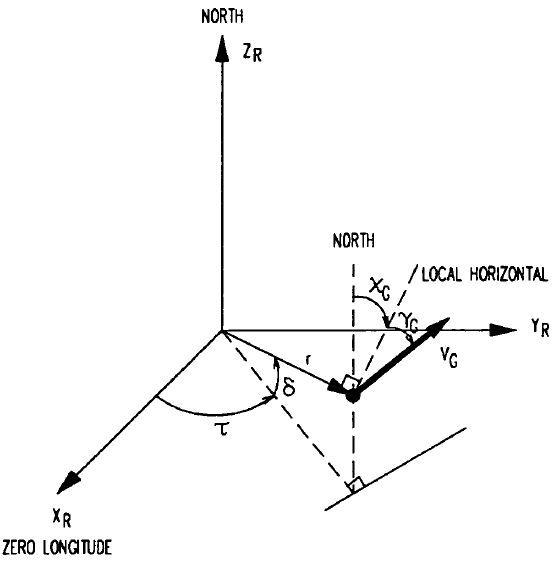
\includegraphics[width=0.7\textwidth]{figures/tsi/spherical_mooij1994motion.jpg}
\caption{Definition of the Spherical coordinates \citep{mooij1994motion}.}
\label{fig:spherical_mooij1994motion}
\end{figure}

\begin{align} \label{eq:spherVecDef}
\begin{split}
\mathbf{R} &= 
\begin{pmatrix}
r \\
\delta \\
\tau \\
\end{pmatrix}
\end{split}
&
\begin{split}
\mathbf{V} &= 
\begin{pmatrix}
V_{G} \\
\gamma_{G} \\
\chi_{G} \\
\end{pmatrix}
\end{split}
&
\begin{split}
m_{MAV}
\end{split}
\end{align}

The different variables are now defined as shown by \Cref{eq:spherVar} and the derivatives by \Cref{eq:spherVarD}. The numbers that were given to the variables are a result of the early derivations.

\begin{align} \label{eq:spherVar}
\begin{split}
x_{16} &= r = h+R_{MOLA} \\
x_{12} &= \delta \\
x_{11} &= \tau \\
\end{split}
&
\begin{split}
x_{15} &= V_{G} \\
x_{14} &= \gamma_{G} \\
x_{13} &= \chi_{G} \\
\end{split}
&
\begin{split}
x_{7} &= m_{MAV} \\
\end{split}
\end{align}

\begin{align} \label{eq:spherVarD}
\begin{split}
x'_{16} &= \dot{r} \\
x'_{12} &= \dot{\delta} \\
x'_{11} &= \dot{\tau} \\
\end{split}
&
\begin{split}
x'_{15} &= \dot{V}_{G} \\
x'_{14} &= \dot{\gamma}_{G} \\
x'_{13} &= \dot{\chi}_{G} \\
\end{split}
&
\begin{split}
x'_{7} &= \dot{m}_{MAV} = -\dfrac{T}{g_{0}I_{sp}} \\
\end{split}
\end{align}

The derivatives given in \Cref{eq:spherVarD} are already provided by \cite{mooij1994motion} in the rotating frame and include the rotational effects. A simplified form can be seen in \Cref{eq:kinEqSp,eq:dynEqSp}. This is why it was decided to perform the \ac{TSI} for the Spherical case in the rotating frame. At the end of the integration the variables can then be transformed to the inertial frame for comparison.

\begin{align} \label{eq:kinEqSp}
\begin{split}
x'_{16} &= \dot{r} = V_{G} s \gamma_{G} \\
\end{split}
&
\begin{split}
x'_{12} &= \dot{\delta} = \dfrac{V_{G} c \chi_{G} c \gamma_{G}}{r} \\
\end{split}
&
\begin{split}
x'_{11} &= \dot{\tau} = \dfrac{V_{G} s \chi_{G} c \gamma_{G}}{r c \delta} \\
\end{split}
\end{align}


\begin{equation} \label{eq:dynEqSp}
\begin{split}
x'_{15} &= \dot{V}_{G} =  \Omega_{M}^{2} r c\delta \left(s\gamma_{G}c\delta-c\gamma_{G}s\delta c\chi_{G}\right)+\dfrac{Tc\psi_{T}c\epsilon_{T}}{m}-\dfrac{D}{m}-\dfrac{\mu_{M}}{r^{2}}s\gamma_{G} \\
x'_{14} &= \dot{\gamma}_{G} = 2\Omega_{M}c\delta s\chi_{G} + \dfrac{V_{G}}{r}c\gamma_{G}+\dfrac{\Omega_{M}^{2}r c\delta}{V_{G}}\left(c\delta c\gamma_{G}+s\gamma_{G} s\delta c\chi_{G}\right)+\dfrac{T s\epsilon_{T}}{V_{G}m}-\dfrac{\mu_{M}}{V_{G}r^{2}}c\gamma_{G} \\
x'_{13} &= \dot{\chi}_{G} = 2 \Omega_{M} \left(s\delta-\dfrac{c\delta s\gamma_{G} c\chi_{G}}{c \gamma_{G}}\right)+\dfrac{V_{G}}{r}c\gamma_{G}\dfrac{s\delta}{c \delta}s\chi_{G}+\dfrac{\Omega_{M}^{2}r c\delta s\delta s\chi_{G}}{V_{G}c\gamma_{G}}+\dfrac{T s\psi_{T}c\epsilon_{T}}{V_{G}m c\gamma_{G}} \\
\end{split}
\end{equation}

The last term in the first two expressions of \Cref{eq:dynEqSp} correspond to the acceleration contribution of the gravity. The first expression has a drag component and all three have a thrust component similar to the Cartesian cases. The rest of the terms come from the rotational effects. In this case it was decided to define the drag as an auxiliary equation $x_{27}$, which will be discussed in more detail later in this section.

\subsubsection{Auxiliary functions for the Spherical case}
\label{subsubsec:auxFspher}
Before the auxiliary functions for \Cref{eq:kinEqSp,eq:kinEqSp} can be written, some standard auxiliary functions have to be defined first. These include $\delta$, $\gamma_{G}$ and $\chi_{G}$. The numbering is based on early derivations and do not correspond to the definitions provided for the Cartesian cases! The angle auxiliary functions are defined in \Cref{eq:SpherAnglF}.

\begin{align} \label{eq:SpherAnglF}
\begin{split}
w_{4,4} &= s\delta = s x_{12}  \\
w_{4,5} &= c\chi_{G} = c x_{13} \\
w_{4,6} &= c\delta = c x_{12} \\
\end{split}
&
\begin{split}
w_{4,7} &= s\gamma_{G} = s x_{14} \\
w_{4,8} &= c\gamma_{G} = c x_{14} \\
w_{4,9} &= s\chi_{G} = s x_{13} \\
\end{split}
\end{align}


Some expression for the thrust are also required. These are similar to the equations defined in \Cref{subsubsec:tsiThrust} but are repeated in \Cref{eq:thrustAuxF} for convenience. 

\begin{align} \label{eq:thrustAuxF}
\begin{split}
w_{4,26} &= \cos \psi_{T} \\
w_{4,27} &= \cos \epsilon_{T} \\
\end{split}
&
\begin{split}
w_{4,28} &= \sin \psi_{T} \\
w_{4,29} &= \sin \epsilon_{T} \\
\end{split}
&
\begin{split}
w_{4,32} &= \dfrac{1}{x_{7}} \\
\end{split}
\end{align}


Now the auxiliary functions can be written for $x'_{11} = u_{11}$ till $x'_{16} = u_{16}$ and are shown in \Cref{eq:auxF11,eq:auxF12,eq:auxF13,eq:auxF14,eq:auxF15,eq:auxF16} respectively. 

\begin{align} \label{eq:auxF11}
\begin{split}
w_{11,0} &= V_{G}c\gamma_{G} = x_{15}w_{4,8} \\
w_{11,1} &= \dfrac{w_{11,0}}{r} = \dfrac{w_{11,0}}{x_{16}} \\
\end{split}
&
\begin{split}
w_{11,2} &= w_{11,1}s\chi_{G} = w_{11,1}w_{4,9} \\
w_{11,3} &= \dfrac{w_{11,2}}{c\delta} = \dfrac{w_{11,2}}{w_{4,6}} \\
\end{split}
&
\begin{split}
u_{11} &= w_{11,3} \\
\end{split}
\end{align}

\begin{align} \label{eq:auxF12}
\begin{split}
w_{12,1} &= w_{11,1}c\chi_{G} = w_{11,1}w_{4,5} \\
\end{split}
&
\begin{split}
u_{12} &= w_{12,1} \\
\end{split}
\end{align}

\begin{align} \label{eq:auxF13}
\begin{split}
w_{13,0} &= s\psi_{T} c\epsilon_{T} = w_{4,28}w_{4,27} \\
w_{13,1} &= s\gamma_{G} c\chi_{G} = w_{4,7}w_{4,5} \\
w_{13,2} &= \Omega_{M}^{2} r c\delta = \Omega_{M}^{2} x_{16} w_{4,6} \\
w_{13,3} &= w_{13,2} s\delta = w_{13,2}w_{4,4} \\
w_{13,4} &= \dfrac{T w_{13,0}}{x_{7}} = T w_{13,0} w_{4,32} \\
\end{split}
&
\begin{split}
w_{13,5} &= w_{13,3} s\chi_{G}+w_{13,4} = w_{13,3}w_{4,9}+w_{13,4} \\
w_{13,6} &= \dfrac{w_{13,5}}{V_{G}} = \dfrac{w_{13,5}}{x_{15}} \\
w_{13,7} &= -2\Omega_{M} c\delta w_{13,1}+w_{13,6} = -2\Omega_{M}w_{4,6}w_{13,1}+w_{13,6} \\
w_{13,8} &= \dfrac{w_{13,7}}{c\gamma_{G}} = \dfrac{w_{13,7}}{w_{4,8}} \\
w_{13,9} &= \left(2\Omega_{M}+w_{11,3} \right) s\delta+w_{13,8} = \left(2\Omega_{M}+w_{11,3} \right)w_{4,4}+w_{13,8} \\
\end{split}
&
\begin{split}
u_{13} &= w_{13,9} \\
\end{split}
\end{align}

\begin{align} \label{eq:auxF14}
\begin{split}
w_{14,0} &= \dfrac{T s\epsilon_{T}}{x_{7}} = T w_{4,29}w_{4,32} \\
w_{14,1} &= c\delta c\gamma_{G}+w_{13,1} s\delta = w_{4,6}w_{4,8}+w_{13,1}w_{4,4} \\
w_{14,2} &= -\mu_{M} c\gamma_{G} = -\mu_{M}w_{4,8} \\
w_{14,3} &= r^{2} = x_{16}^{2} \\
w_{14,4} &= \dfrac{w_{14,2}}{w_{14,3}} \\
\end{split}
&
\begin{split}
w_{14,5} &= w_{14,4}+w_{13,2}w_{14,1}+w_{14,0} \\
w_{14,6} &= \dfrac{w_{14,5}}{V_{G}} = \dfrac{w_{14,5}}{x_{15}} \\
w_{14,7} &= 2\Omega_{M}c\delta s\chi_{G}+w_{11,1}+w_{14,6} = 2\Omega_{M}w_{4,6}w_{4,9}+w_{11,1}+w_{14,6} \\
\\
u_{14} &= w_{14,7} \\
\end{split}
\end{align}

\begin{align} \label{eq:auxF15}
\begin{split}
w_{15,0} &= T c\psi_{T} c\epsilon_{T}-D = Tw_{4,26}w_{4,27}-x_{27} \\
w_{15,1} &= \dfrac{w_{15,0}}{m_{MAV}} = \dfrac{w_{15,0}}{x_{7}} \\
w_{15,2} &= -\mu_{M} s\gamma_{G} = -\mu_{M}w_{4,7} \\
w_{15,3} &= \dfrac{w_{15,2}}{w_{14,3}} \\
\end{split}
&
\begin{split}
w_{15,4} &= c\gamma_{G}c\chi_{G} = w_{4,8}w_{4,5} \\
w_{15,5} &= s\gamma_{G} c\delta - w_{15,4} s\delta = w_{4,7}w_{4,6}-w_{15,4}w_{4,4} \\
w_{15,6} &= w_{13,2}w_{15,5}+w_{15,1}+w_{15,3} \\
\\
u_{15} &= w_{15,6} \\
\end{split}
\end{align}

\begin{align} \label{eq:auxF16}
\begin{split}
w_{16,1} &= V_{G} s\gamma_{G} = x_{15}w_{4,7} \\
\end{split}
&
\begin{split}
u_{16} &= w_{16,1} \\
\end{split}
\end{align}




 
 \subsubsection{Drag acceleration as auxiliary variable}
 \label{subsubsec:tsiDragAuxE}
The drag acceleration for the Spherical case is similar to the Cartesian case, except this time it was chosen to use auxiliary variables to describe the drag. This means that auxiliary equations have to be defined as is shown in \Cref{eq:dragAux}. Also, this means that auxiliary derivatives are required for each of these equations. \Cref{eq:dragDerAux} shows the different derivatives corresponding to the equations.
 
 \begin{equation} \label{eq:dragAux}
\begin{split}
x_{27} &= D = \frac{1}{2}\rho V_{G}^{2}SC_{D} = \frac{1}{2}Sx_{28}x_{15}^{2}x_{29}\\
x_{28} &= \rho = e^{x_{30}} \\
x_{29} &= C_{D} \\
x_{30} &= P_{\rho 10}x_{31}^{10}+P_{\rho 9}x_{31}^{9}+P_{\rho 8}x_{31}^{8}+P_{\rho 7}x_{31}^{7}+P_{\rho 6}x_{31}^{6}+P_{\rho 5}x_{31}^{5}+P_{\rho 4}x_{31}^{4}+P_{\rho 3}x_{31}^{3}+P_{\rho 2}x_{31}^{2}+P_{\rho 1}x_{31}+P_{\rho 0} \\
x_{31} &= h = r-R_{MOLA} = x_{16}-R_{MOLA} \\
\end{split}
\end{equation}

 \begin{equation} \label{eq:dragDerAux}
\begin{split}
x'_{27} &= \frac{1}{2}Sx_{15}\left(x_{15} \left(x_{29}x'_{28}+x_{28}x'_{29}\right)+2x_{28}x_{29}x'_{15}\right) \\
x'_{28} &= x'_{30}x_{28} \\
x'_{30} &=x'_{31} \left(10 P_{\rho 10}x_{31}^{9}+9 P_{\rho 9}x_{31}^{8}+8 P_{\rho 8}x_{31}^{7}+7 P_{\rho 7}x_{31}^{6}+6 P_{\rho 6}x_{31}^{5}+\dots \right. \\
&  \left. \dotsc +5 P_{\rho 5}x_{31}^{4}+4 P_{\rho 4}x_{31}^{3}+3 P_{\rho 3}x_{31}^{2}+2 P_{\rho 2}x_{31}+P_{\rho 1}\right) \\
x'_{31} &= x'_{16}
\end{split}
\end{equation}

The auxiliary derivatives described in \Cref{eq:dragDerAux} can now be used to define the auxiliary functions. These are described in \Cref{eq:u27,eq:u28,eq:u30} for $u_{27}$, $u_{28}$ and $u_{30}$ respectively. In this case $u_{31}=u_{16}$.

\begin{align} \label{eq:u27}
\begin{split}
w_{27,1} &= C_{D}\dot{\rho} = x_{29}u_{28} \\
w_{27,2} &= \rho \dot{C}_{D} = x_{28}u_{29} \\
w_{27,3} &= \rho C_{D} = x_{28}x_{29} \\
\end{split}
&
\begin{split}
w_{27,4} &= V_{G}\left(w_{27,1}+w_{27,2}\right) = x_{15}\left(w_{27,1}+w_{27,2}\right) \\
w_{27,5} &= w_{27,3}\dot{V}_{G} = w_{27,3}u_{15} \\
w_{27,6} &= V_{G}\left(w_{27,4}+w_{27,5}\right) = x_{15}\left(w_{27,4}+w_{27,5}\right) \\
\end{split}
&
\begin{split}
u_{27} &= \frac{1}{2} S w_{27,6}\\
\end{split}
\end{align}

\begin{align} \label{eq:u28}
\begin{split}
w_{28,1} &= u_{30}\rho = u_{30}x_{28} \\
\end{split}
&
\begin{split}
u_{28} &= w_{28,1} \\
\end{split}
\end{align}

\begin{align} \label{eq:u30}
\begin{split}
w_{30,1} &= h^{9} = x_{31}^9 \\
w_{30,2} &= h^{8} = x_{31}^8 \\
w_{30,3} &= h^{7} = x_{31}^7 \\
w_{30,4} &= h^{6} = x_{31}^6 \\
w_{30,5} &= h^{5} = x_{31}^5 \\
\end{split}
&
\begin{split}
w_{30,6} &= h^{4} = x_{31}^4 \\
w_{30,7} &= h^{3} = x_{31}^3 \\
w_{30,8} &= h^{2} = x_{31}^2 \\
w_{30,9} &= u_{31}\left(10P_{\rho 10}w_{30,1}+\dots +3P_{\rho 3}w_{30,8} + 2P_{\rho 2}x_{31}+P_{\rho 1}\right) \\
\\
u_{30} &= w_{30,9} \\
\end{split}
\end{align}

Again, three additional auxiliary equations are required for the $C_{D}-M$ relation (see \Cref{fig:dragcoeff_whitehead2004mars}) and are presented in \Cref{eq:cdAux}.

 \begin{equation} \label{eq:cdAux}
\begin{split}
x_{32} &= M = \dfrac{V_{G}}{a} = \dfrac{x_{15}}{x_{33}}\\
x_{33} &= a = \sqrt{\gamma_{a}R_{a}^{*}T_{a}} = \sqrt{\gamma_{a}R_{a}^{*}x_{34}} \quad \text{where} \quad R_{a}^{*}=\dfrac{R_{a}}{M_{a}} \\
x_{34} &= T_{a}
\end{split}
\end{equation}

In this case the conditional relations shown in \Cref{eq:cdCond} are not used directly in the recurrence relations, but only serve as initial conditions. Again, the $P_{C_{D} number,section}$ are the polynomial fit coefficients as provided in \Cref{tab:dragCoeffPara}.

\begin{equation}\label{eq:cdCond}
x_{29}=C_{D}=\begin{cases}
x_{29,1}=0.2, & \text{for } 0\leq x_{32} < 0.5\\
x_{29,2}=P_{C_{D} 1,2}x_{32}+P_{C_{D} 0,2}, &  \text{for } 0.5\leq x_{32} < 1 \\
x_{29,3}=P_{C_{D} 1,3}x_{32}+P_{C_{D} 0,3}, &  \text{for } 1\leq x_{32} < 1.3 \\
x_{29,4}=P_{C_{D} 1,4}x_{32}+P_{C_{D} 0,4}, &  \text{for } 1.3\leq x_{32} < 2.5 \\
x_{29,5}=P_{C_{D} 1,5}x_{32}+P_{C_{D} 0,5}, &  \text{for } 2.5\leq x_{32} < 4 \\
x_{29,6}=0.3, &  \text{for } x_{32} \geq 4 
\end{cases}\\
\end{equation}

The corresponding derivatives that will have to be used for the recurrence relations are presented in \Cref{eq:cdCondDer}.

\begin{equation}\label{eq:cdCondDer}
x'_{29}=\begin{cases}
x'_{29,1}=0, & \text{for } 0\leq x_{32} < 0.5\\
x'_{29,2}=P_{C_{D} 1,2}x'_{32}, &  \text{for } 0.5\leq x_{32} < 1 \\
x'_{29,3}=P_{C_{D} 1,3}x'_{32}, &  \text{for } 1\leq x_{32} < 1.3 \\
x'_{29,4}=P_{C_{D} 1,4}x'_{32}, &  \text{for } 1.3\leq x_{32} < 2.5 \\
x'_{29,5}=P_{C_{D} 1,5}x'_{32}, &  \text{for } 2.5\leq x_{32} < 4 \\
x'_{29,6}=0, &  \text{for } x_{32} \geq 4 
\end{cases}\\
\end{equation}

The Mach derivative and corresponding speed of sound derivative are then described in \Cref{eq:cdDerAux}.

 \begin{equation} \label{eq:cdDerAux}
\begin{split}
x'_{32} &= \dfrac{x_{33}x'_{15}-x_{15}x'_{33}}{x_{33}^{2}}\\
x'_{33} &= \dfrac{\gamma_{a}R_{a}^{*}}{2x_{33}}x'_{34} 
\end{split}
\end{equation}

For the drag coefficient, there are no auxiliary functions required. That is why $x'$ in \Cref{eq:cdCondDer} can simply be replaced by $u$. The Mach number and the speed of sound do require auxiliary functions and are described in \Cref{eq:u32,eq:u33} respectively.

\begin{align} \label{eq:u32}
\begin{split}
w_{32,1} &= a\dot{V}_{G} = x_{33}u_{15} \\
w_{32,2} &= V_{G}\dot{a} = x_{15}u_{33} \\
\end{split}
&
\begin{split}
w_{32,3} &= a^{2} = x_{33}^2 \\
w_{32,4} &= \dfrac{w_{32,1}-w_{32,2}}{w_{32,3}} \\
\end{split}
&
\begin{split}
u_{32} &= w_{32,4} \\
\end{split}
\end{align}

\begin{align} \label{eq:u33}
\begin{split}
w_{33,1} &= \dfrac{\dot{T}_{a}}{a} = \dfrac{u_{34}}{x_{33}} \\
\end{split}
&
\begin{split}
u_{33} &= w_{33,1} \\
\end{split}
\end{align}

The last relations that still need to be described are the ones for the temperature $T_{a}$. Similar to $C_{D}$ the corresponding auxiliary equations, shown by \Cref{eq:tempCondAux} are only used for the initial conditions. Again, $P_{T number,section}$ are the polynomial fit coefficients as provided in \Cref{tab:fitParameters}.

\begin{equation}\label{eq:tempCondAux}
x_{34}=T_{a}=\begin{cases}
x_{34,1}=P_{T 1,1}x_{31}+P_{T 0,1}, & \text{for } -0.6 \leq x_{31} < 5.04  \\
x_{34,2}=P_{T 3,2}x_{31}^{3}+P_{T 2,2}x_{31}^{2}+P_{T 1,2}x_{31}+P_{T 0,2}, &  \text{for } 5.04 \leq x_{31} < 35.53   \\
x_{34,3}=P_{T 6,3}x_{31}^{6}+P_{T 5,3}x_{31}^{5}+P_{T 4,3}x_{31}^{4}+P_{T 3,3}x_{31}^{3}+ \dots \\
\qquad\ \ \dotsc +P_{T 2,3}x_{31}^{2}+P_{T 1,3}x_{31}+P_{T 0,3}, &  \text{for } 35.53 \leq x_{31} < 75.07   \\
x_{34,4}=P_{T 8,4}x_{31}^{8}+P_{T 7,4}x_{31}^{7}+P_{T 6,4}x_{31}^{6}+P_{T 5,4}x_{31}^{5} \\
\qquad\ \ +P_{T 4,4}x_{31}^{4}+P_{T 3,4}x_{31}^{3}+P_{T 2,4}x_{31}^{2}+P_{T 1,4}x_{31}+P_{T 0,4}, &  \text{for } 75.07 \leq x_{31} < 170.05   \\
x_{34,5}=136.5, &  \text{for }  x_{31} \geq 170.05   
\end{cases}
\end{equation}

The corresponding derivatives that are used for the recurrence relations are presented in \Cref{eq:TCondDerAux}.

\begin{equation}\label{eq:TCondDerAux}
x'_{34}=\begin{cases}
x'_{34,1}=P_{T 1,1}x'_{31}, & \text{for } -0.6 \leq x_{31} < 5.04  \\
x'_{34,2}=\left(3P_{T 3,2}x_{31}^{2}+2P_{T 2,2}x_{31}+P_{T 1,2}\right)x'_{31}, &  \text{for } 5.04\leq x_{31} < 35.53   \\
x'_{34,3}=\left(6 P_{T 6,3}x_{31}^{5}+5P_{T 5,3}x_{31}^{4}+4P_{T 4,3}x_{31}^{3}+ \dots
\right. \\
\qquad\  \left. \dotsc +3P_{T 3,3}x_{31}^{2}+2P_{T 2,3}x_{31}+P_{T 1,3}\right)x'_{31}, &  \text{for } 35.53\leq x_{31} < 75.07   \\
x'_{34,4}=\left(8 P_{T 8,4}x_{31}^{7}+7P_{T 7,4}x_{31}^{6}+6P_{T 6,4}x_{31}^{5}
+5P_{T 5,4}x_{31}^{4}+ \dots \right. \\
\qquad\  \left. \dotsc +4P_{T 4,4}x_{31}^{3}+3P_{T 3,4}x_{31}^{2}+2P_{T 2,4}x_{31}+P_{T 1,4}\right)x'_{31}, &  \text{for } 75.07\leq x_{31} < 170.05   \\
x'_{34,5}=0, &  \text{for }  x_{31} \geq 170.05   
\end{cases}
\end{equation}

All the power relations in \Cref{eq:TCondDerAux} were already described in auxiliary functions in \Cref{eq:u30}. Therefore, depending on the section, the equations presented in \Cref{eq:TCondDerAux} can be rewritten by simply replacing $x'$ by $u$ and the auxiliary functions. This is shown in \Cref{eq:TCondAuxF}.

\begin{equation}\label{eq:TCondAuxF}
u_{34}=\begin{cases}
u_{34,1}=P_{T 1,1}u_{31}, & \text{for } -0.6 \leq x_{31} < 5.04  \\
u_{34,2}=\left(3P_{T 3,2}w_{30,2}+2P_{T 2,2}x_{31}\right)u_{31}+P_{T 1,2}u_{31}, &  \text{for } 5.04\leq x_{31} < 35.53   \\
u_{34,3}=\left(6 P_{T 6,3}w_{30,5}+5P_{T 5,3}w_{30,4}+4P_{T 4,3}w_{30,3}+ \dots
\right. \\
\qquad\  \left. \dotsc +3P_{T 3,3}w_{30,2}+2P_{T 2,3}x_{31}\right)u_{31}+P_{T 1,3}u_{31}, &  \text{for } 35.53\leq x_{31} < 75.07   \\
u_{34,4}=\left(8 P_{T 8,4}w_{30,7}+7P_{T 7,4}w_{30,6}+6P_{T 6,4}w_{30,5}
+5P_{T 5,4}w_{30,4}+ \dots \right. \\
\qquad\  \left. \dotsc +4P_{T 4,4}w_{30,3}+3P_{T 3,4}w_{30,2}+2P_{T 2,4}x_{31}\right)u_{31}+P_{T 1,4}u_{31}, &  \text{for } 75.07\leq x_{31} < 170.05   \\
u_{34,5}=0, &  \text{for }  x_{31} \geq 170.05   
\end{cases}
\end{equation}

Now all the information that is required to compute the recurrence relation for the drag is available. Please note that there is a certain order in which these equations have to be computed, since they depend on each other. \Cref{tab:calcOrderAuxEq} shows this order.


\begin{table}[!ht]
\begin{center}
\caption{Order of auxiliary equations and derivatives computations}
\label{tab:calcOrderAuxEq}
\begin{tabular}{|l|l||l|l||l|l||l|l|}
\hline 
\multicolumn{4}{c}{\textbf{Auxiliary equations}} & \multicolumn{4}{c}{\textbf{Auxiliary derivatives}} \\ \hline \hline
\textbf{Order} & $\mathbf{x_{n}}$ &\textbf{Order} & $\mathbf{x_{n}}$ & \textbf{Order} & $\mathbf{u_{n}}$ & \textbf{Order} & $\mathbf{u_{n}}$ \\ \hline 
0 & $ x_{7} ,x_{11}, x_{12}, x_{13}, x_{14}, x_{15}, x_{16} $ & 4 & $ x_{32}$ & 7 & $ u_{7}, u_{11}, u_{12}, u_{16} $ & 11 & $ u_{32} $  \\ \hline
1 & $ x_{31} $ & 5 & $ x_{29} $  & 8 & $u_{31}$ &  12 &  $ u_{29} $ \\ \hline
2 & $ x_{30}, x_{34}$ & 6 & $ x_{27} $  & 9 & $ u_{30}, u_{34} $ &  13 & $ u_{27} $ \\ \hline
3 & $ x_{33}, x_{28} $ &   &  & 10 & $ u_{28}, u_{33} $ &  14 &  $ u_{13}, u_{14}, u_{15} $\\ \hline


\end{tabular}
\end{center}
\end{table}





%
%
% \textbf{\textcolor{red}{Rest still has to be rewritten!!}}



\subsection{Recurrence relations}
\label{subsec:recRel}
Now that all the auxiliary functions are known, they can be used to determine the required recurrence relations. In order to write these concisely and following the same convention as used by \cite{scott2008high}, a number of extra parameters will have to be introduced. The Taylor series coefficients can be written as described by \Cref{eq:tsCoeff}. Where $n$ is the variable number and $k$ is the order of the derivative.

\begin{equation} \label{eq:tsCoeff}
\dfrac{x_{n}^{\left(k\right)}}{k!} \triangleq X_{n}\left(k\right) \quad \text{where} \quad k \geq 1
\end{equation}

A similar expression is defined for $u_{n}$ and $w_{n}$ as well as the place-holder functions $f_{n}$ and $g_{n}$ which are all shown in \Cref{eq:redDer}.

\begin{align} \label{eq:redDer}
U_{n}\left(k\right)& \triangleq \dfrac{u_{n}^{\left(k\right)}}{k!}
&
W_{n}\left(k\right)& \triangleq \dfrac{w_{n}^{\left(k\right)}}{k!}
&
F_{n}\left(k\right)& \triangleq \dfrac{f_{n}^{\left(k\right)}}{k!}
&
G_{n}\left(k\right)& \triangleq \dfrac{g_{n}^{\left(k\right)}}{k!}
\end{align}



Then remembering that $u_{n}=x'_{n}$ and using \Cref{eq:tsCoeff} a relation can be described between $X_{n}$ and $U_{n}$ as shown in \Cref{eq:UnXn} \citep{scott2008high}. 

\begin{equation} \label{eq:UnXn}
\begin{split}
u_{n}^{\left( k-1\right)}=x_{n}^{\left( k\right)} \quad &\Rightarrow \quad \dfrac{u_{n}^{\left( k-1\right)}}{\left(k-1\right)!} = \dfrac{x_{n}^{\left( k\right)}}{\left(k-1\right)!} \quad \Rightarrow\\
U_{n}\left(k-1\right)=kX_{n}\left(k\right) \quad &\Rightarrow \quad X_{n}\left(k\right)=\dfrac{U_{n}\left(k-1\right)}{k}
\end{split}
\end{equation}

Using these definitions, the auxiliary functions can be written into reduced auxiliary functions $W\left(k\right)$ for the three cases. The equations stay the same, but the lower-case letters are replaced by their upper-case counterparts. A complete list of the reduced auxiliary functions (starting at $k=2$, or the second derivative $u'$) for the three cases is presented in \Cref{app:appendixD-allRecurrenceRelations}.
As was mentioned before, all the auxiliary functions have been defined such that they incorporate one of the following operations: multiplication, division, power, exponential or trigonometric. This has been done because recurrence relations exist for these simple operations as provided by \cite{jorba2005software}. These recurrence relations are written using the definitions from \Cref{eq:redDer} and are described in \Cref{eq:recRel1,eq:recRel2,eq:recRel3,eq:recRel4,eq:recRel5,eq:recRel6,eq:recRel7}.

\begin{equation} \label{eq:recRel1}
\text{for} \quad f_{n} \pm g_{n} \quad \Rightarrow \quad W_{n,\pm}\left(k\right)= F_{n}\left(k\right) \pm G_{n}\left(k\right)
\end{equation}

\begin{equation} \label{eq:recRel2}
\text{for} \quad f_{n}g_{n} \quad \Rightarrow \quad W_{n,mult}\left(k\right)=\displaystyle\sum_{j=0}^{k}F_{n}\left(j\right)G_{n}\left(k-j\right)
\end{equation}

\begin{equation} \label{eq:recRel3}
\text{for} \quad \dfrac{f_{n}}{g_{n}} \quad \Rightarrow \quad W_{n,div}\left(k\right)= \dfrac{1}{G_{n}\left(0\right)}\left[F_{n}\left(k\right)-\displaystyle\sum_{j=1}^{k}G_{n}\left(j\right)W_{n,div}\left(k-j\right) \right]
\end{equation}

\begin{equation} \label{eq:recRel4}
\text{for} \quad f_{n}^{\alpha} \quad \Rightarrow \quad W_{n,pow}\left(k\right)= \dfrac{1}{kF_{n}\left(0\right)} \displaystyle\sum_{j=0}^{k-1}\left[k\alpha-j\left(\alpha+1\right)\right] F_{n}\left(k-j\right)W_{n,pow}\left(j\right) 
\end{equation}

\begin{equation} \label{eq:recRel5}
\text{for} \quad e^{f_{n}} \quad \Rightarrow \quad W_{n,exp}\left(k\right)= \dfrac{1}{k}\displaystyle\sum_{j=0}^{k-1}\left(k-j\right)W_{n,exp}\left(j\right)F_{n}\left(k-j\right)
\end{equation}

\begin{equation} \label{eq:recRel6}
\text{for} \quad \cos f_{n} \quad \Rightarrow \quad W_{n,cos}\left(k\right)= -\dfrac{1}{k}\displaystyle\sum_{j=1}^{k}jW_{n,sin}\left(k-j\right)F_{n}\left(j\right)
\end{equation}

\begin{equation} \label{eq:recRel7}
\text{for} \quad \sin f_{n}  \quad \Rightarrow \quad W_{n,sin}\left(k\right)= \dfrac{1}{k}\displaystyle\sum_{j=1}^{k}jW_{n,cos}\left(k-j\right)F_{n}\left(j\right)
\end{equation}

Checking the presented equations it can be seen that \Cref{eq:recRel6,eq:recRel7} are interdependent. This means that whenever a cosine recurrence relation has to be computed, the same recurrence relation for sine (with at least order $k-1$) has to be computed at the same time (and vice versa). All these equations have been derived by \cite{jorba2005software} using the general Leibniz rule for the $k^{th}$ derivative of a multiplication as portrayed in \Cref{eq:Leibniz}.

\begin{equation} \label{eq:Leibniz}
\left(f_{n}g_{n}\right)^{\left( k\right)}=\displaystyle\sum_{j=0}^{k}
\left(
\begin{matrix}
k\\
j\\
\end{matrix}
\right)
f_{n}^{\left( j\right)}g_{n}^{\left( k-j\right)}
\end{equation}

Combining \Cref{eq:Leibniz} and the definition of the reduced derivative for the auxiliary function (see \Cref{eq:redDer}) results in \Cref{eq:LeibnizInt}. This equation, when rewritten to include the reduced derivatives for $f_{n}$ and $g_{n}$, results in \Cref{eq:recRel2}.

\begin{equation} \label{eq:LeibnizInt}
W_{n,mult}\left(k\right)=\dfrac{1}{k!}\displaystyle\sum_{j=0}^{k}
\left(
\begin{matrix}
k\\
j\\
\end{matrix}
\right)
f_{n}^{\left( j\right)}g_{n}^{\left( k-j\right)}
\end{equation}

With all the recurrence relations now known, and using the definition of \Cref{eq:UnXn} the updated state can be described using the Taylor series expansion as described in \Cref{eq:TSexp}.

\begin{equation} \label{eq:TSexp}
x_{n}\left(t+h\right)=\displaystyle\sum_{k=0}^{K}\dfrac{x_{n}^{\left( k\right)}\left(t\right)}{k!}h^{k}+T_{n,K}=\displaystyle\sum_{k=0}^{K}X_{n}\left( k \right) h^{k}+T_{n,K} \quad \text{with }n=1,\dotsc,7
\end{equation}

Here $K$ is the order of the series to which it has to be evaluated and $T_{n,K}$ is the truncation error. Please note that all the Taylor series coefficients computed for the auxiliary equations are only needed to determine the Taylor series coefficients of the state variables (which is why they are auxiliary).

%Maybe change the names of multiplication to product, division to quotient.

%jorba2005software



%
%\subsubsection{Recurrence relations}
%\label{subsubsec:recRel}


%
%\textcolor{red}{\textbf{Get rid of the arctan for $x_{11}$ and replace it with arccos and function of the sqrt of $x_{19}$. $u_{11}$ can remain the same.}}


